\chapter{Additional plots and tables} \label{appB:additional}

%%%%%%%%%%%%%%%%%%%%%%%%%%%%%%%%%%%%%%%%%%%%%%%%%%%%%%%%%%%%%%%%%%%%%%%
%%%%%%%%%%%%%%%%%%%%%%%%%%%%%%%%%%%%%%%%%%%%%%%%%%%%%%%%%%%%%%%%%%%%%%%

\section{Chapter 3: Bayesian estimation} \label{appB1:chapter3}

\subsection{To center or not to center} \label{appB1:noncenter}
%
\begin{figure}[H]
	\centering
	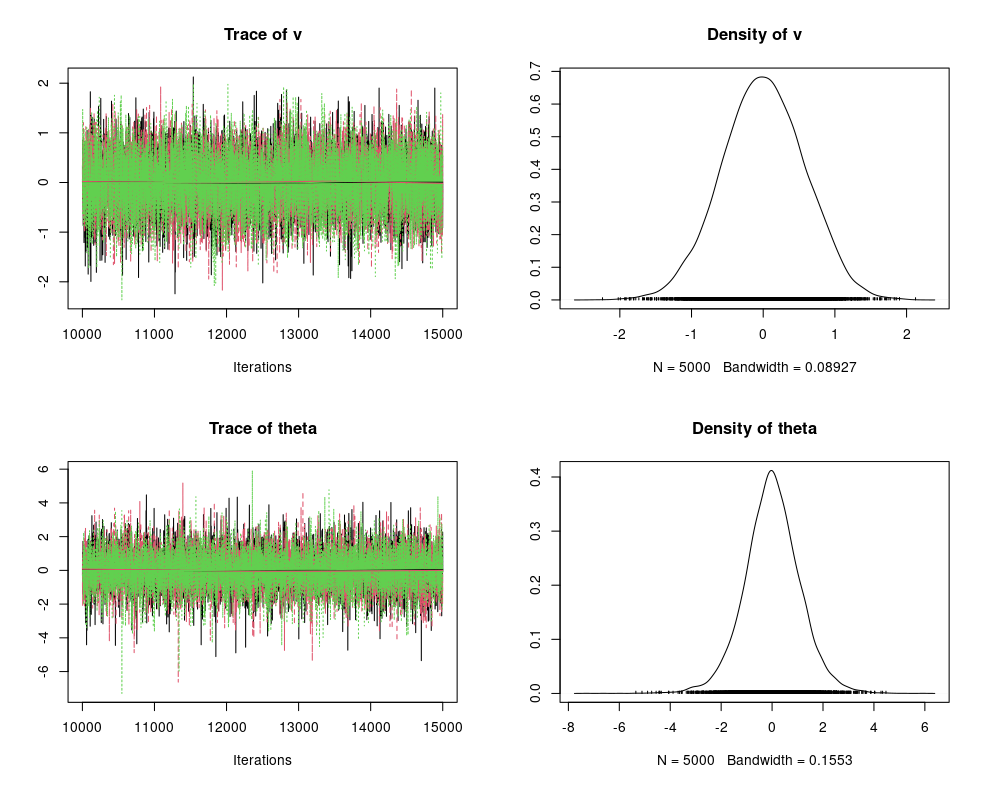
\includegraphics[width=1\linewidth]{1_jags_CE_simple}
	%
	\caption[The Devil's funnel. Centered Parametrization. JAGS]%
	{The Devil's funnel. Centered Parametrization implemented in JAGS. It shows the traceplot and distribution of the parameters of interest.}
	\label{fig:devil_CE_simple_jags}
\end{figure}
%
\begin{figure}[H]
	\centering
	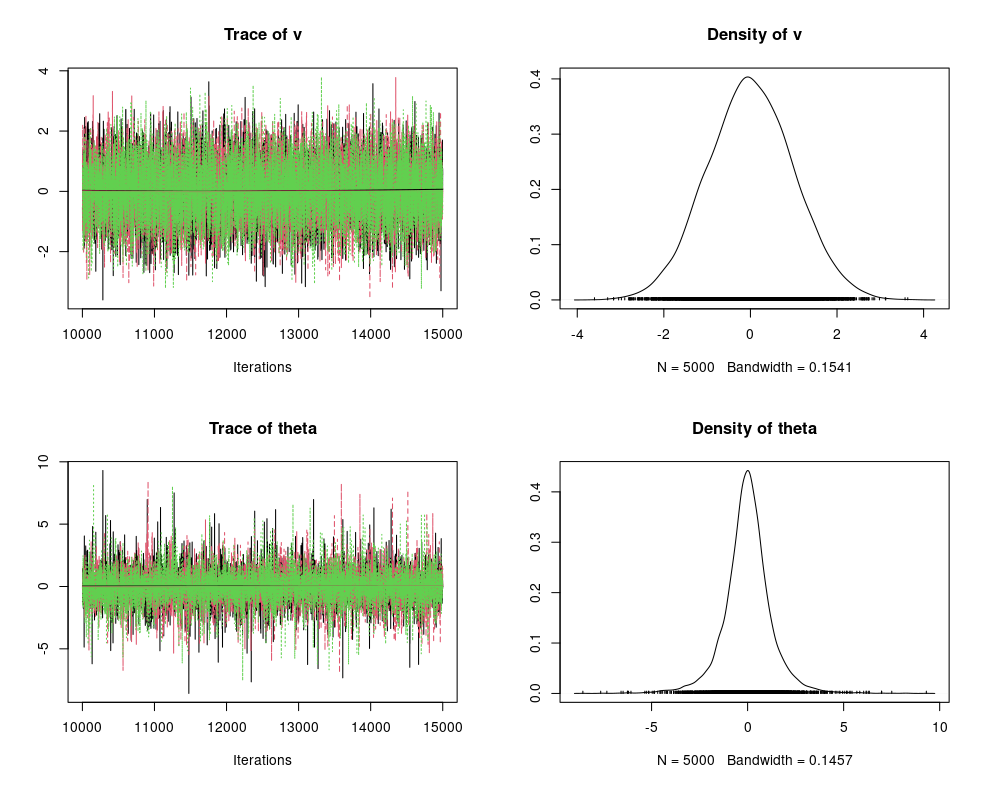
\includegraphics[width=1\linewidth]{2_jags_CE_priors}
	%
	\caption[The Devil's funnel. Centered Parametrization with mildly informative priors. JAGS]%
	{The Devil's funnel. Centered Parametrization with mildly informative priors implemented in JAGS. It shows the traceplot and distribution of the parameters of interest.}
	\label{fig:devil_CE_prior_jags}
\end{figure}
%
\begin{figure}[H]
	\centering
	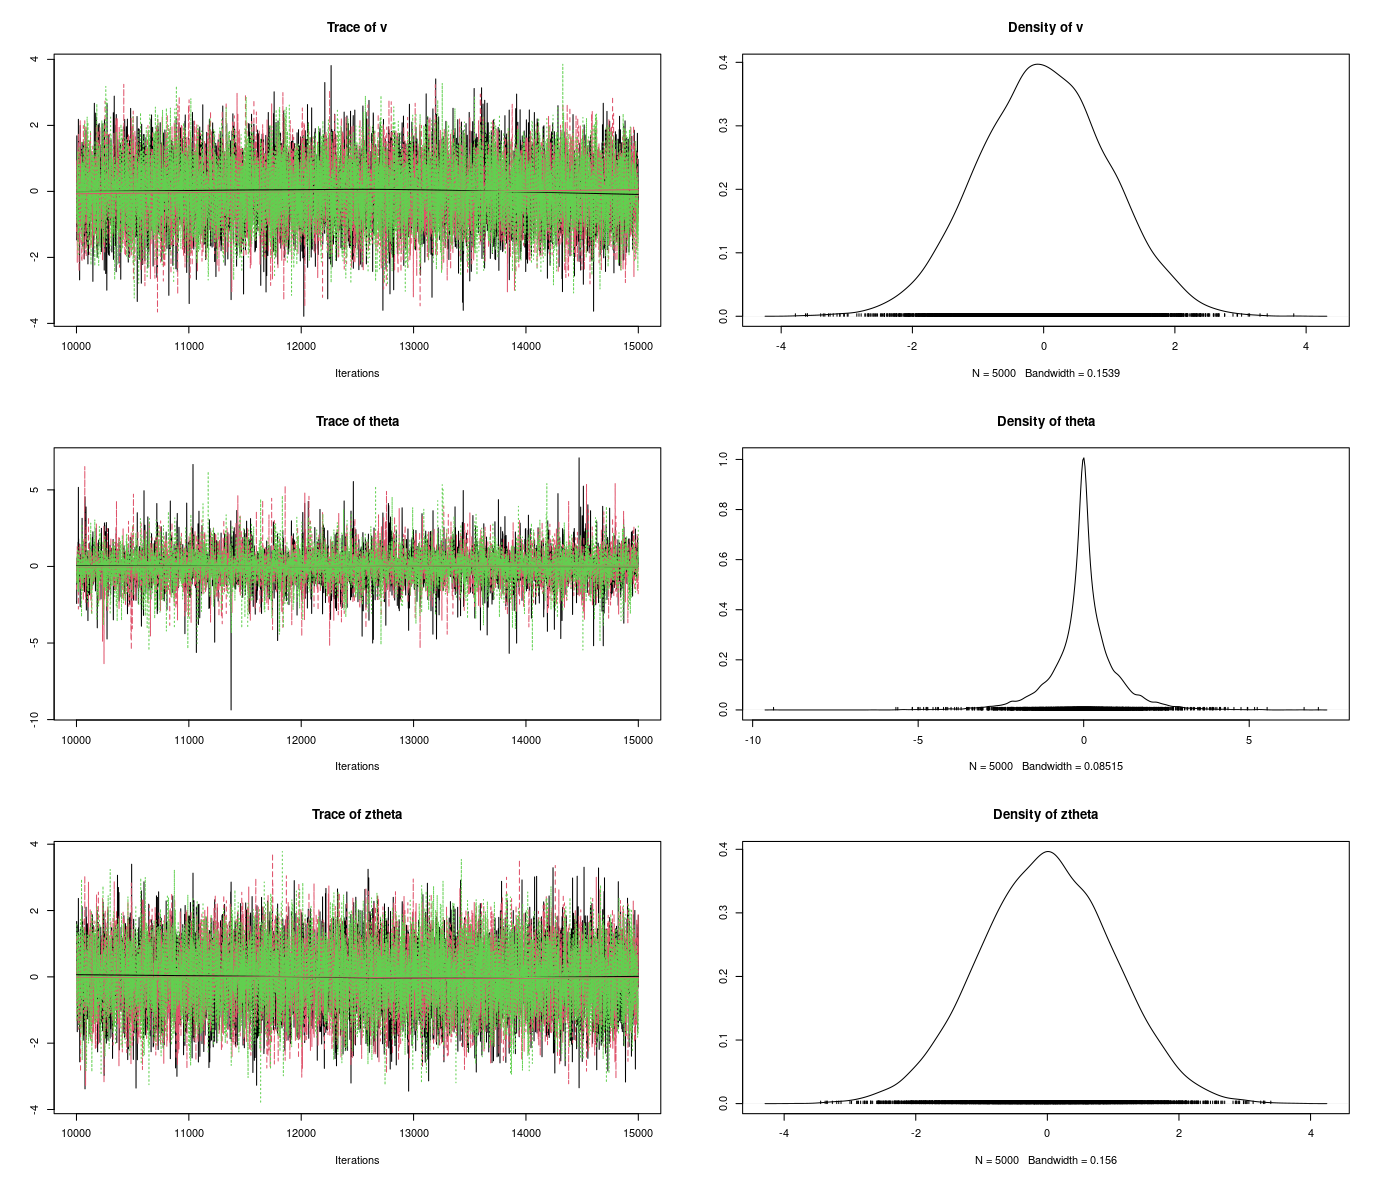
\includegraphics[width=1\linewidth]{3_jags_NC}
	%
	\caption[The Devil's funnel. Non-Centered Parametrization. JAGS]%
	{The Devil's funnel. Non-Centered Parametrization implemented in JAGS. It shows the traceplot and distribution of the parameters of interest.}
	\label{fig:devil_CE_NC_jags}
\end{figure}

%%%%%%%%%%%%%%%%%%%%%%%%%%%%%%%%%%%%%%%%%%%%%%%%%%%%%%%%%%%%%%%%%%%%%%%


%%%%%%%%%%%%%%%%%%%%%%%%%%%%%%%%%%%%%%%%%%%%%%%%%%%%%%%%%%%%%%%%%%%%%%%
%%%%%%%%%%%%%%%%%%%%%%%%%%%%%%%%%%%%%%%%%%%%%%%%%%%%%%%%%%%%%%%%%%%%%%%


\section{Chapter 4: Simulation study} \label{appB2:chapter4}

\subsection{Prior elicitation}
%
\begin{figure}[H]
	\centering
	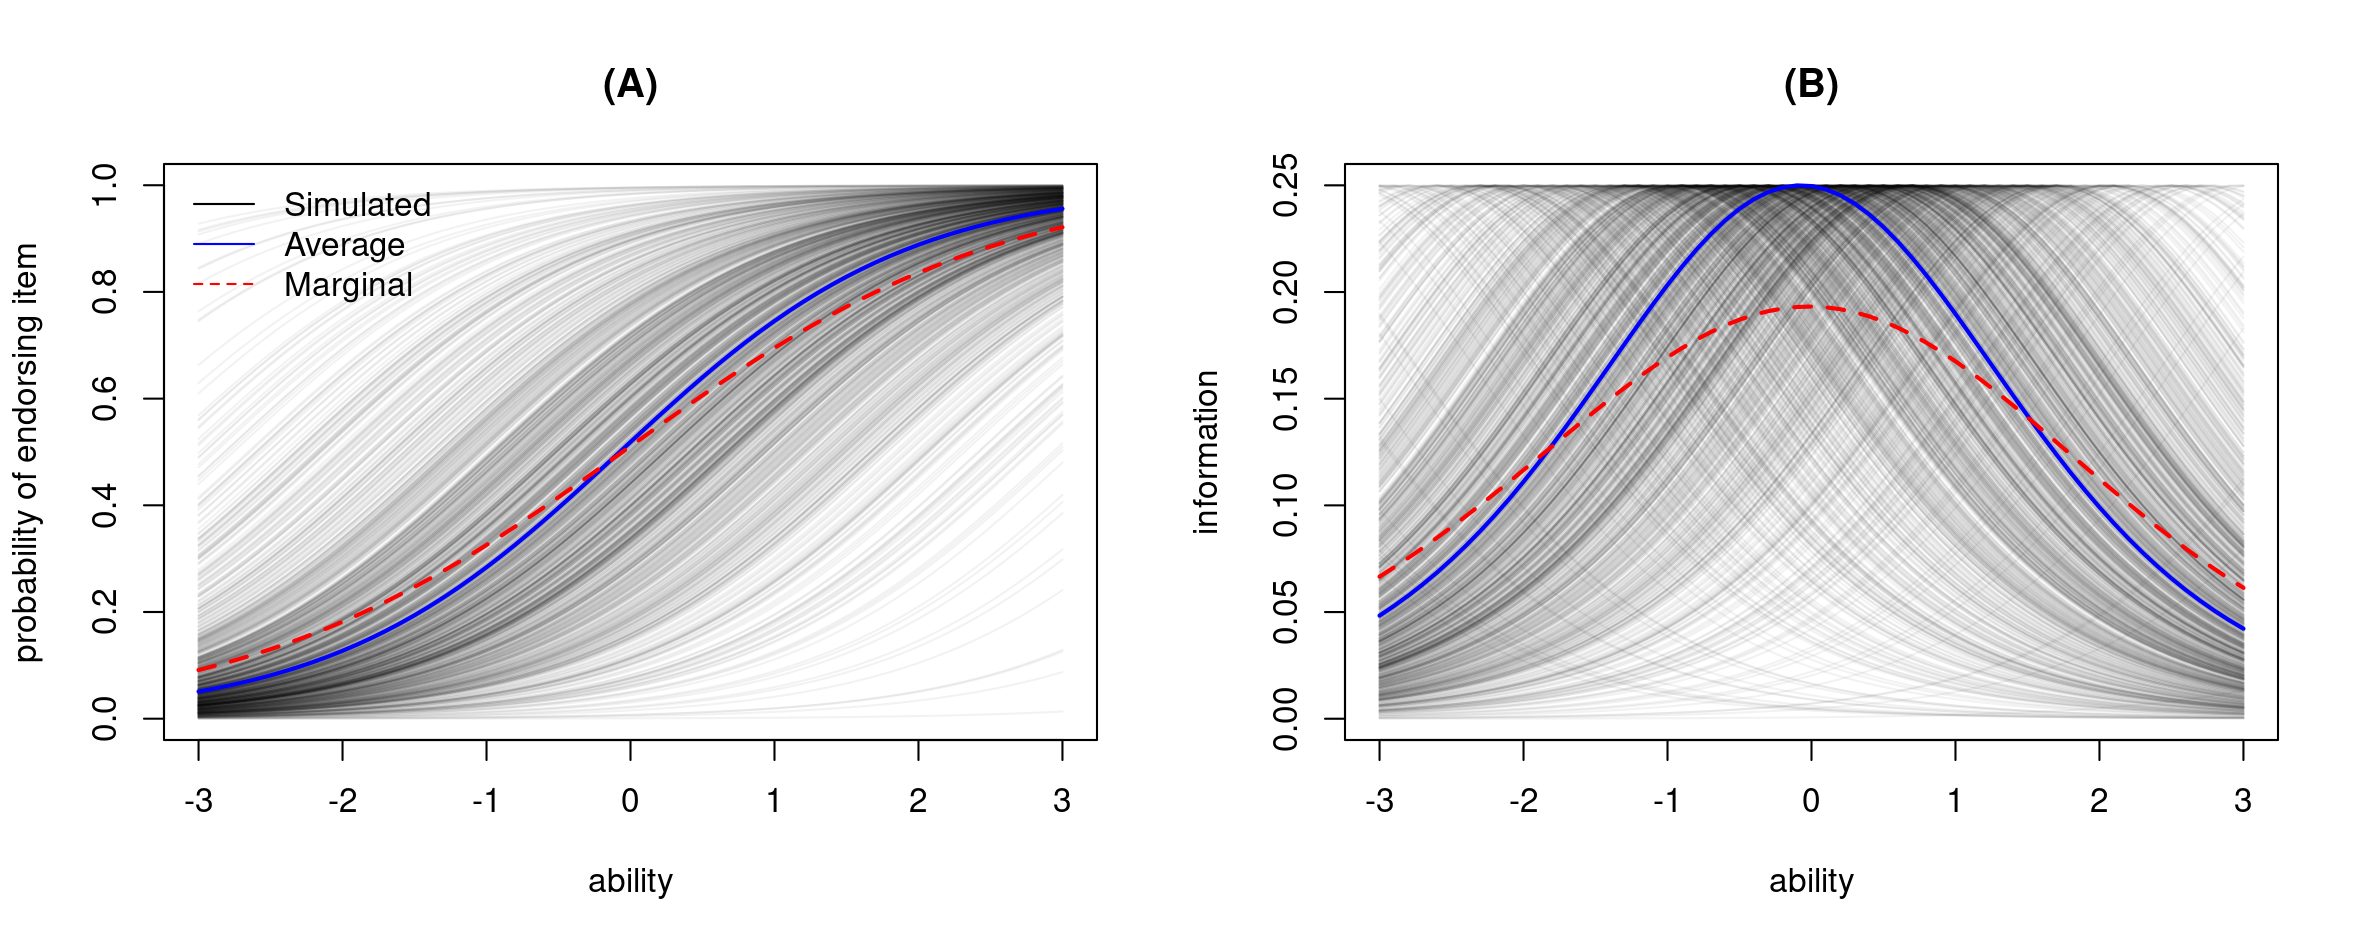
\includegraphics[width=1\linewidth]{SOLV_ICC_prior}
	%
	\caption[Second-Order latent variable model (SOLV). Item Characteristic Curve (ICC) and Item Information Function (IIF).]%
	{Second-Order latent variable model (SOLV). (A) Item Characteristics Curve, ICC. (B) Item Information Function, IIF.}
	\label{fig:SOLV_ICC_prior}
\end{figure}
%
\begin{figure}[H]
	\centering
	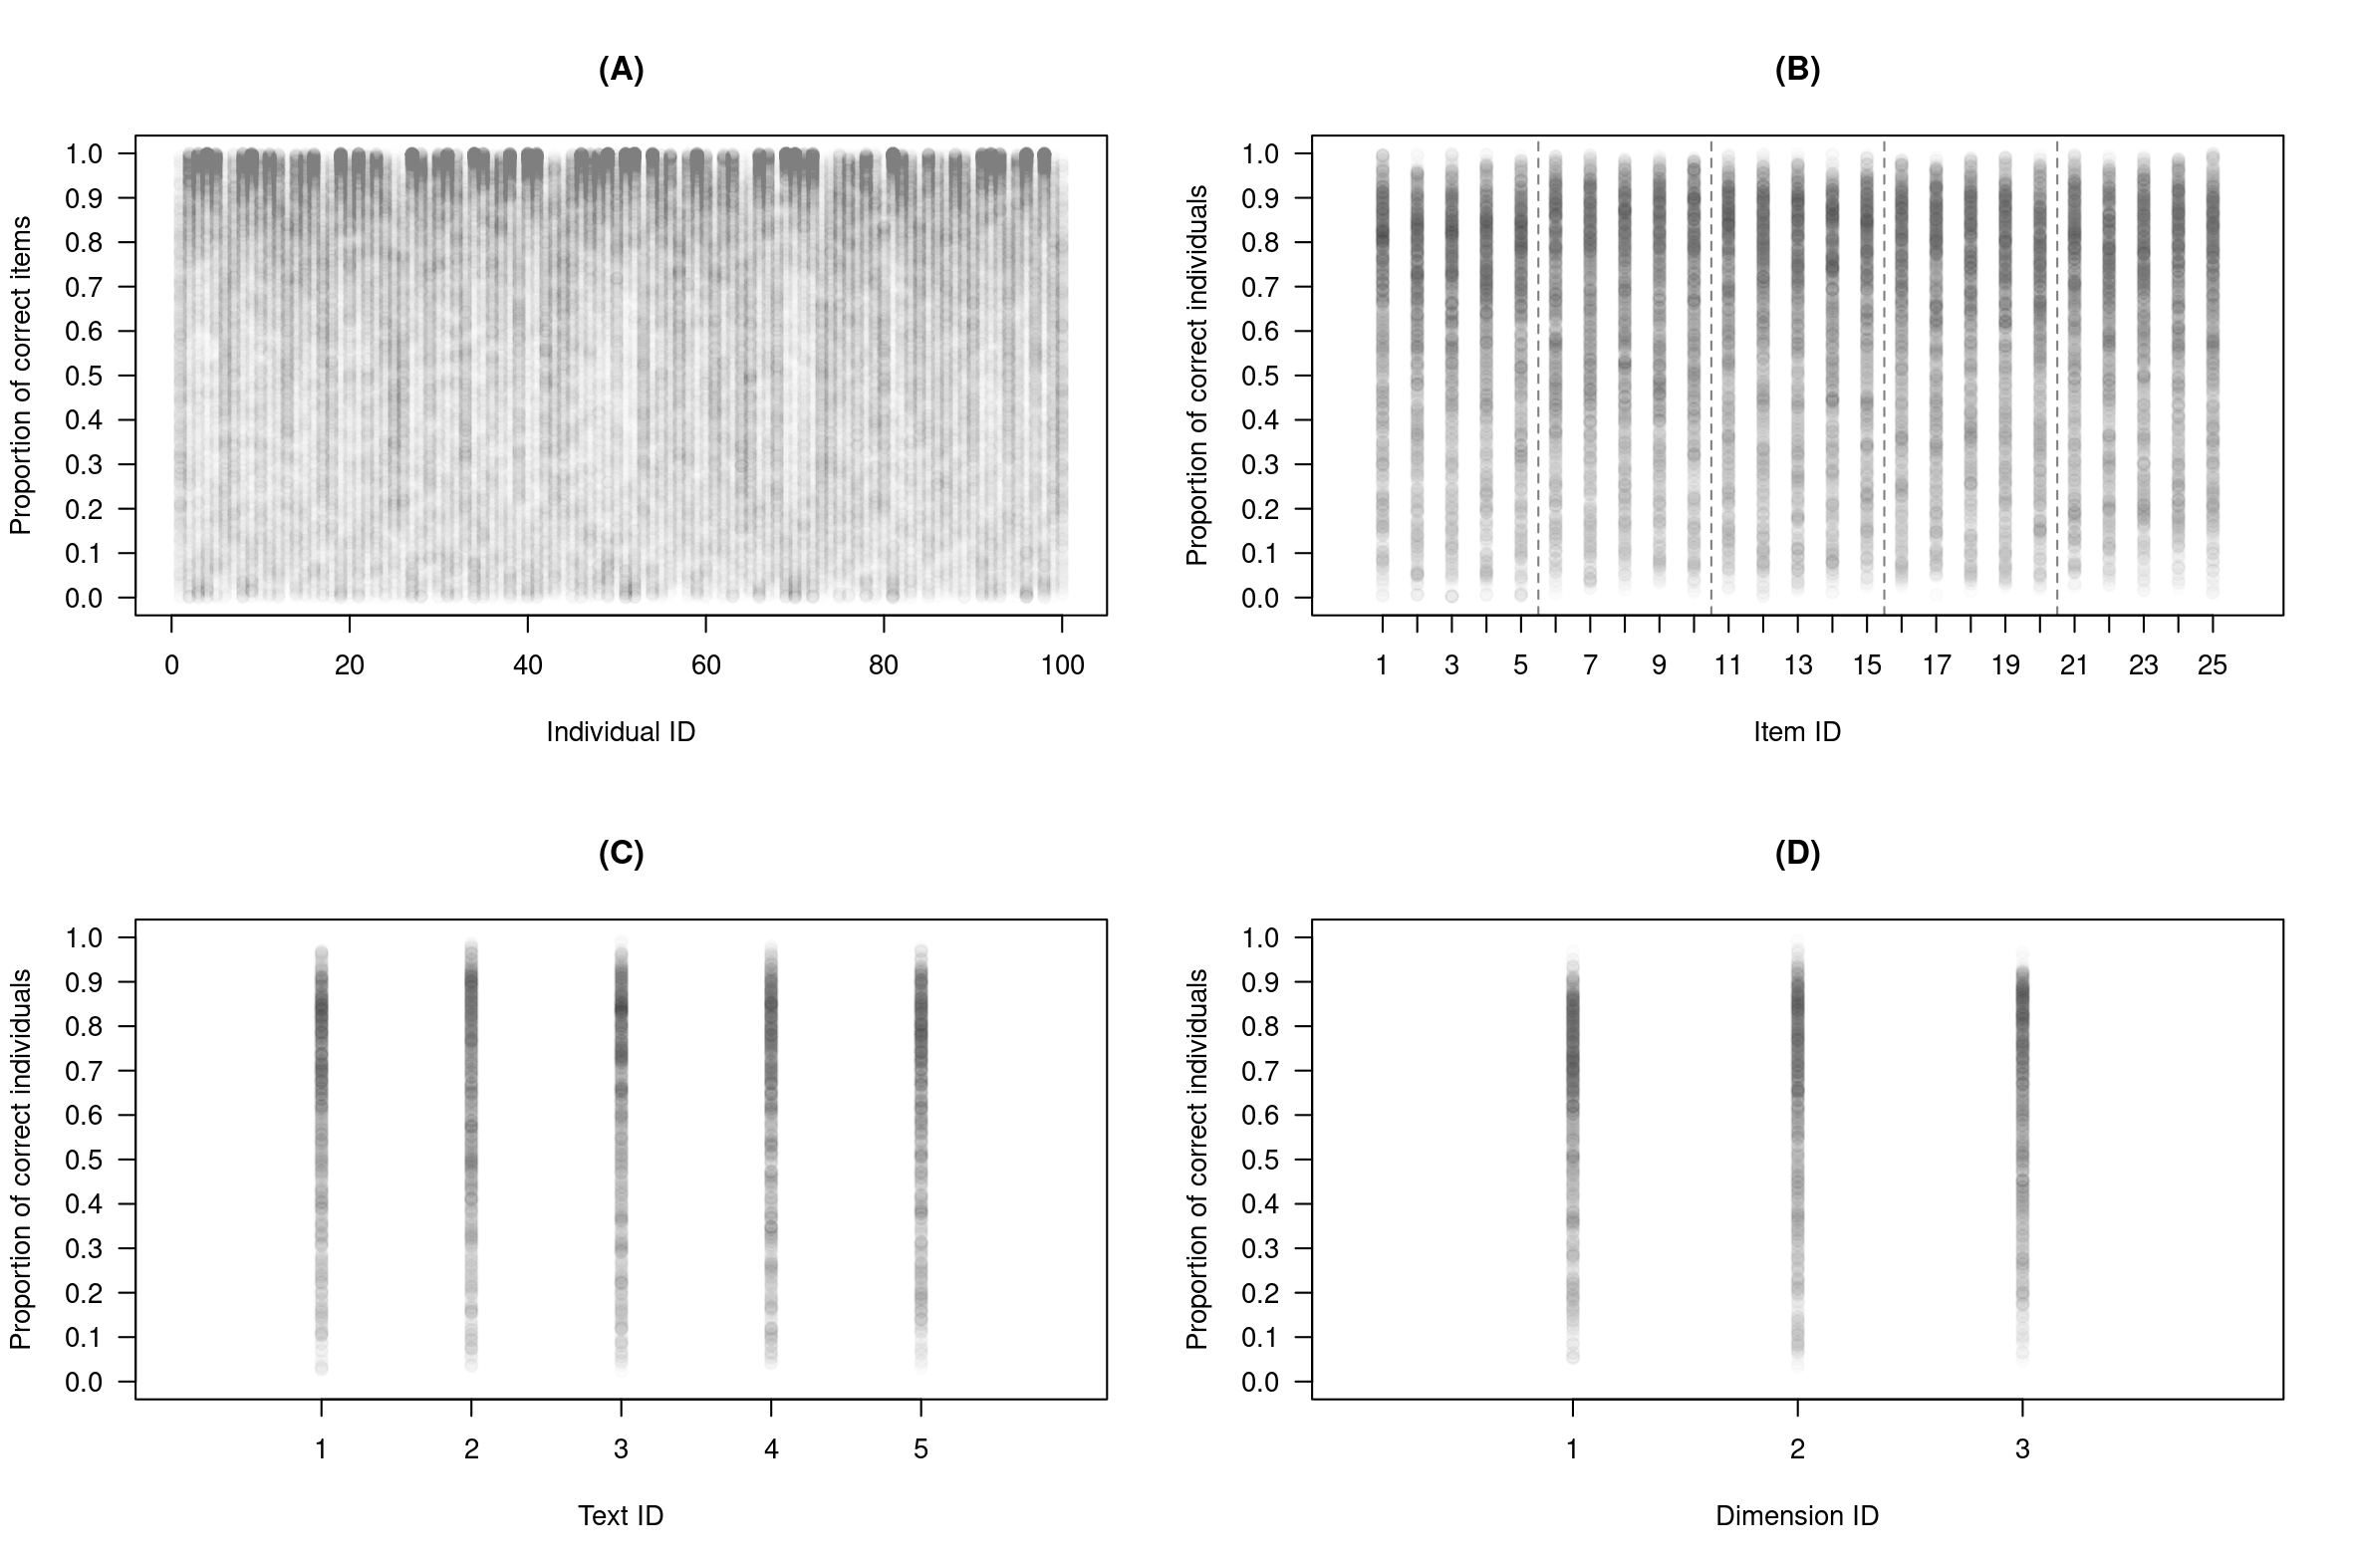
\includegraphics[width=1\linewidth]{SOLV_HitRate1}
	%
	\caption[Second-Order latent variable model (SOLV). Hit rate per dimensions of interest.]%
	{Second-Order latent variable model (SOLV). Aggregated endorsement rate per: (A) individuals, (B) items, (C) text or passage, and (D) measured dimension.}
	\label{fig:SOLV_hitrate1}
\end{figure}
%
\begin{figure}[H]
	\centering
	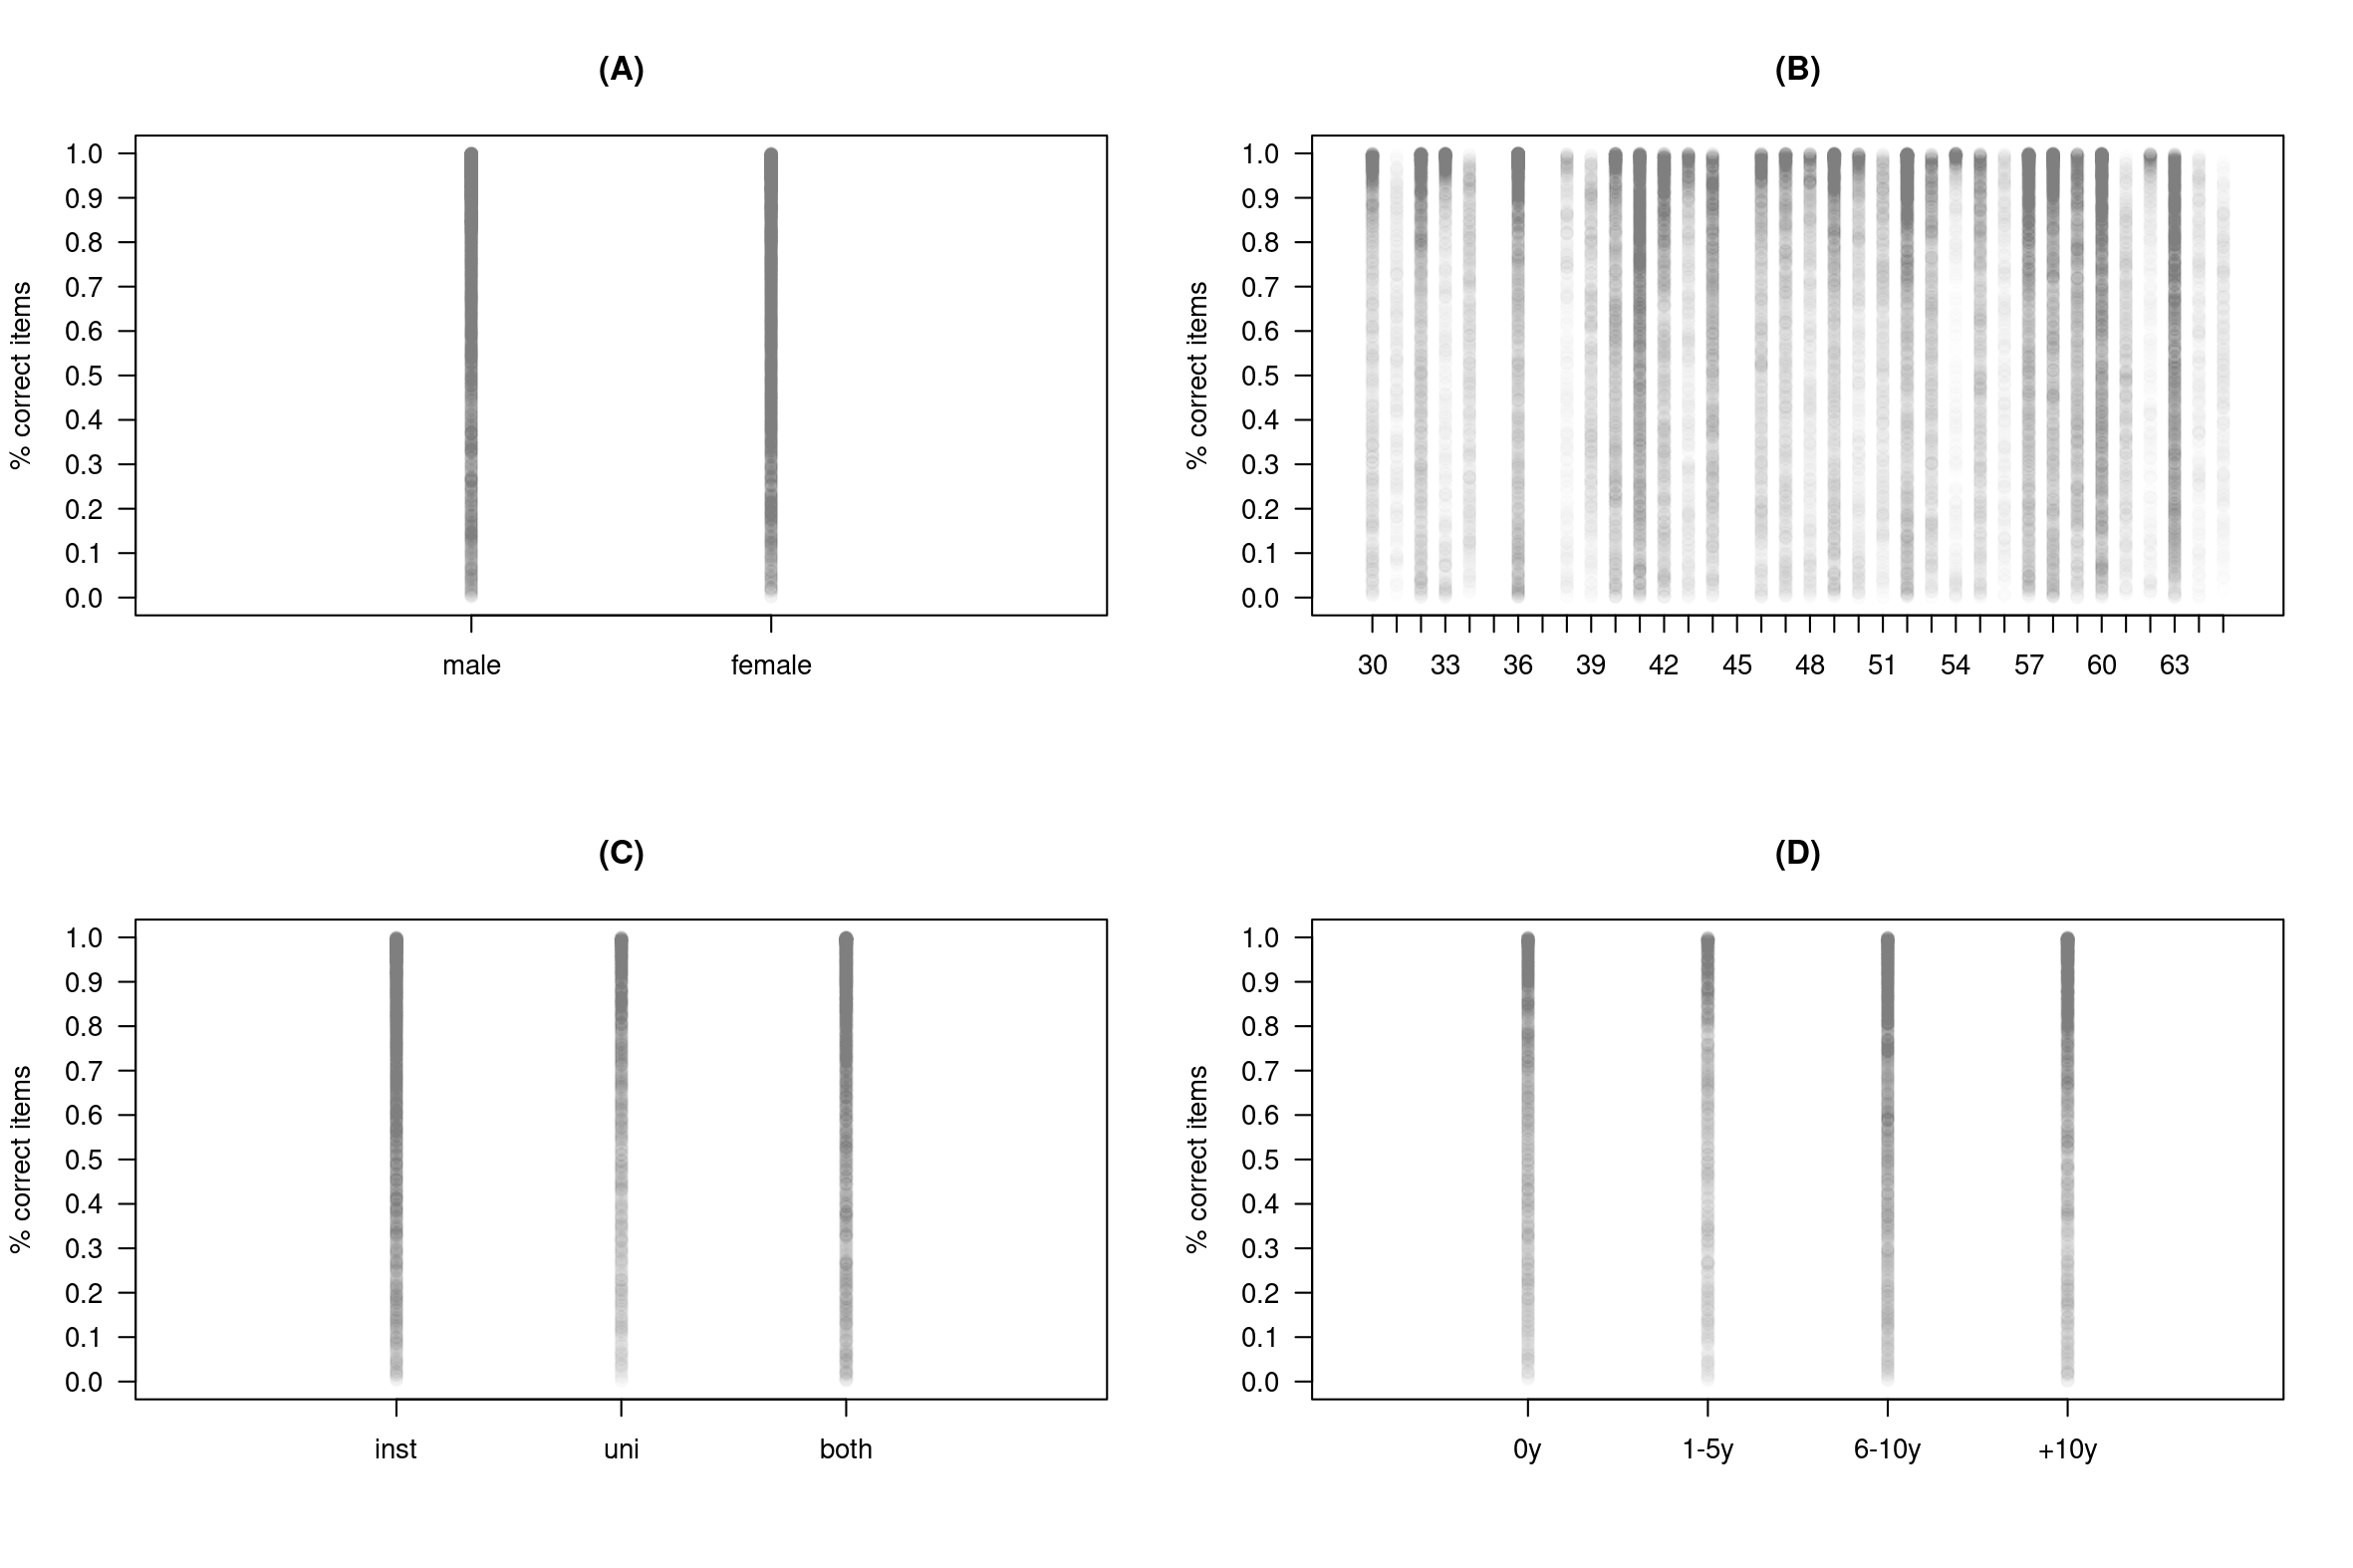
\includegraphics[width=1\linewidth]{SOLV_HitRate2}
	%
	\caption[Second-Order latent variable model (SOLV). Hit rate per simulated covariate.]%
	{Second-Order latent variable model (SOLV). Aggregated endorsement rate per simulated covariate: (A) gender, (B) age, (C) education, and (D) experience.}
	\label{fig:SOLV_hitrate2}
\end{figure}


\subsection{Chain performance}

This section only shows a small set of trace, trank and ACF plots for the parameters of interest. For all the plots across parameters, models, parametrizations, and replicas refer to the images section of the accompanying github page:

\noindent \url{https://github.com/jriveraespejo/thesis/tree/master/images/chains} \\

\noindent Similarly, the CP and NCP \texttt{n\_eff} and \texttt{Rhat} comparison plots shown here is a small set of the full available plots. For the set of figures across parameters, models, and replicas refer to the corresponding image section of the accompanying github page:

\noindent \url{https://github.com/jriveraespejo/thesis/tree/master/images/chains_stat}
%
\begin{figure}[H]
	\centering
	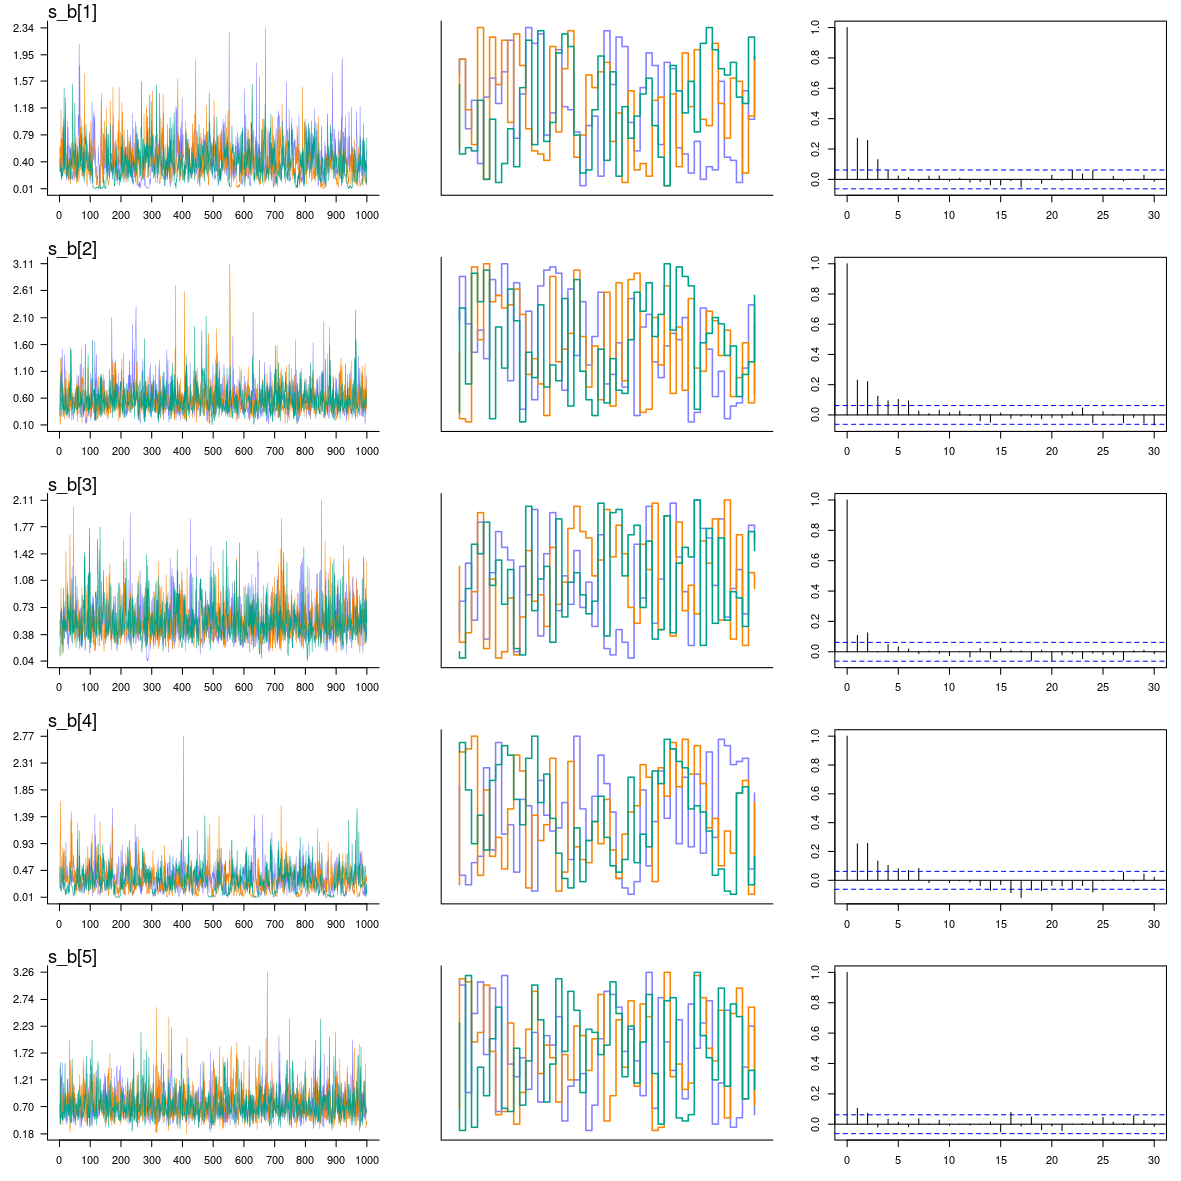
\includegraphics[width=1\linewidth]{FOLV_CE_J100_Ndata3_sb}
	%
	\caption[First-Order latent variable model (FOLV). Sample size $100$, replica number $3$. Centered parametrization. Difficulty deviation per text. Trace, trank and auto-correlation plots.]%
	{First-Order latent variable model (FOLV). Sample size $100$, replica number $3$. Centered parametrization. Difficulty deviation per text: (Left) trace plot, (Middle) trank plot, (Right) auto-correlation plot.}
	\label{fig:FOLV_CE_chains2}
\end{figure}
%
\begin{figure}[H]
	\centering
	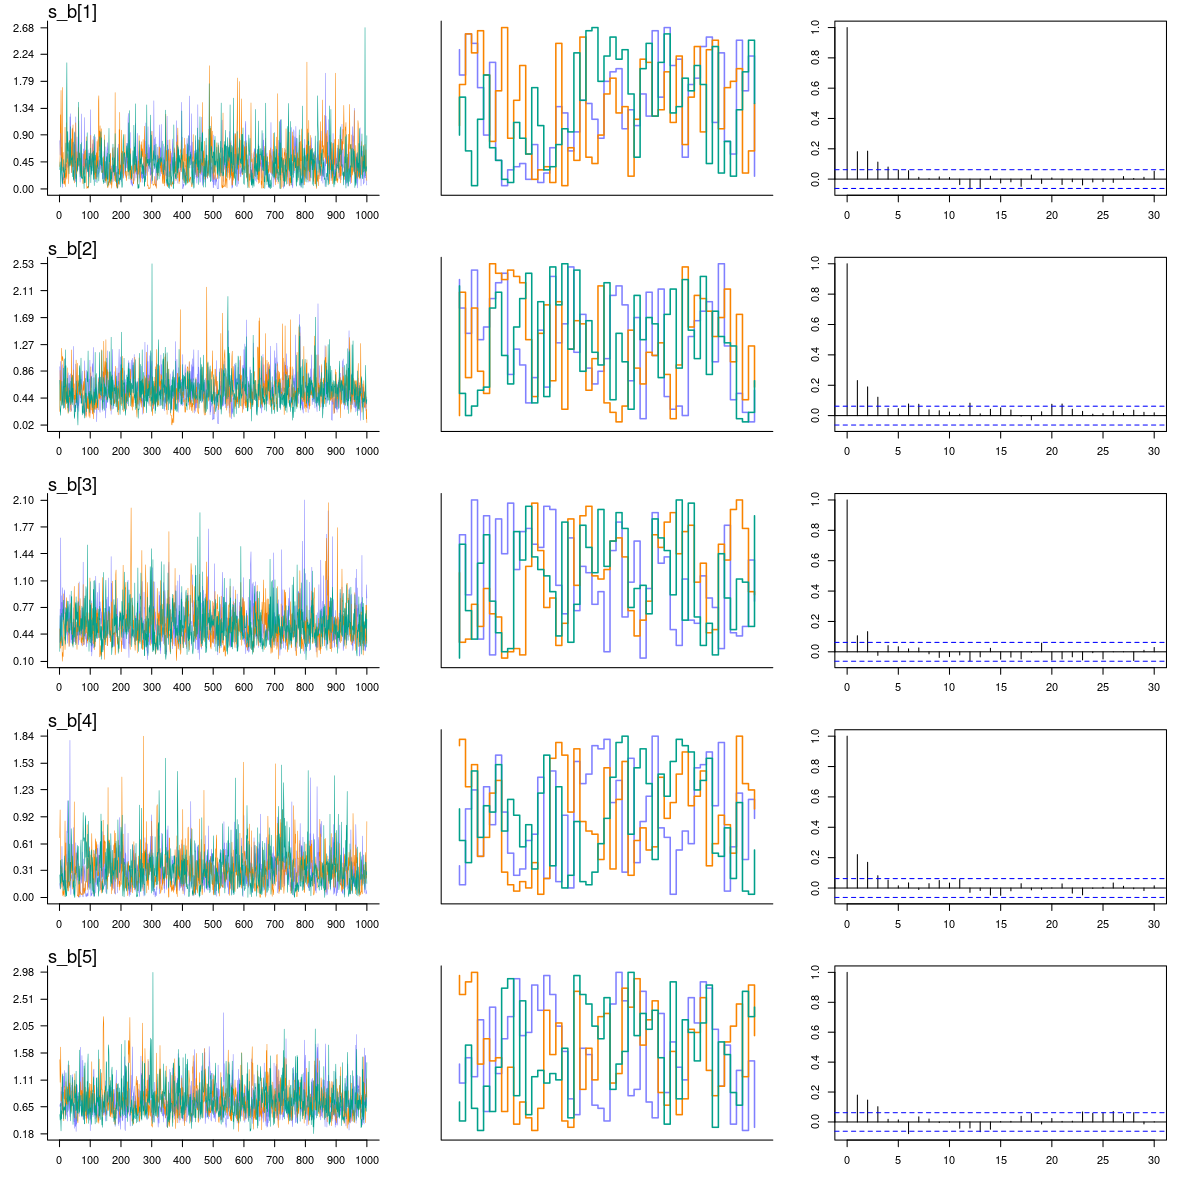
\includegraphics[width=1\linewidth]{FOLV_NC_J100_Ndata3_sb}
	%
	\caption[First-Order latent variable model (FOLV). Sample size $100$, replica number $3$. Non-centered parametrization. Difficulty deviation per text. Trace, trank and auto-correlation plots.]%
	{First-Order latent variable model (FOLV). Sample size $100$, replica number $3$. Non-centered parametrization. Difficulty deviation per text: (Left) trace plot, (Middle) trank plot, (Right) auto-correlation plot.}
	\label{fig:FOLV_NC_chains2}
\end{figure}
%
\begin{figure}[H]
	\centering
	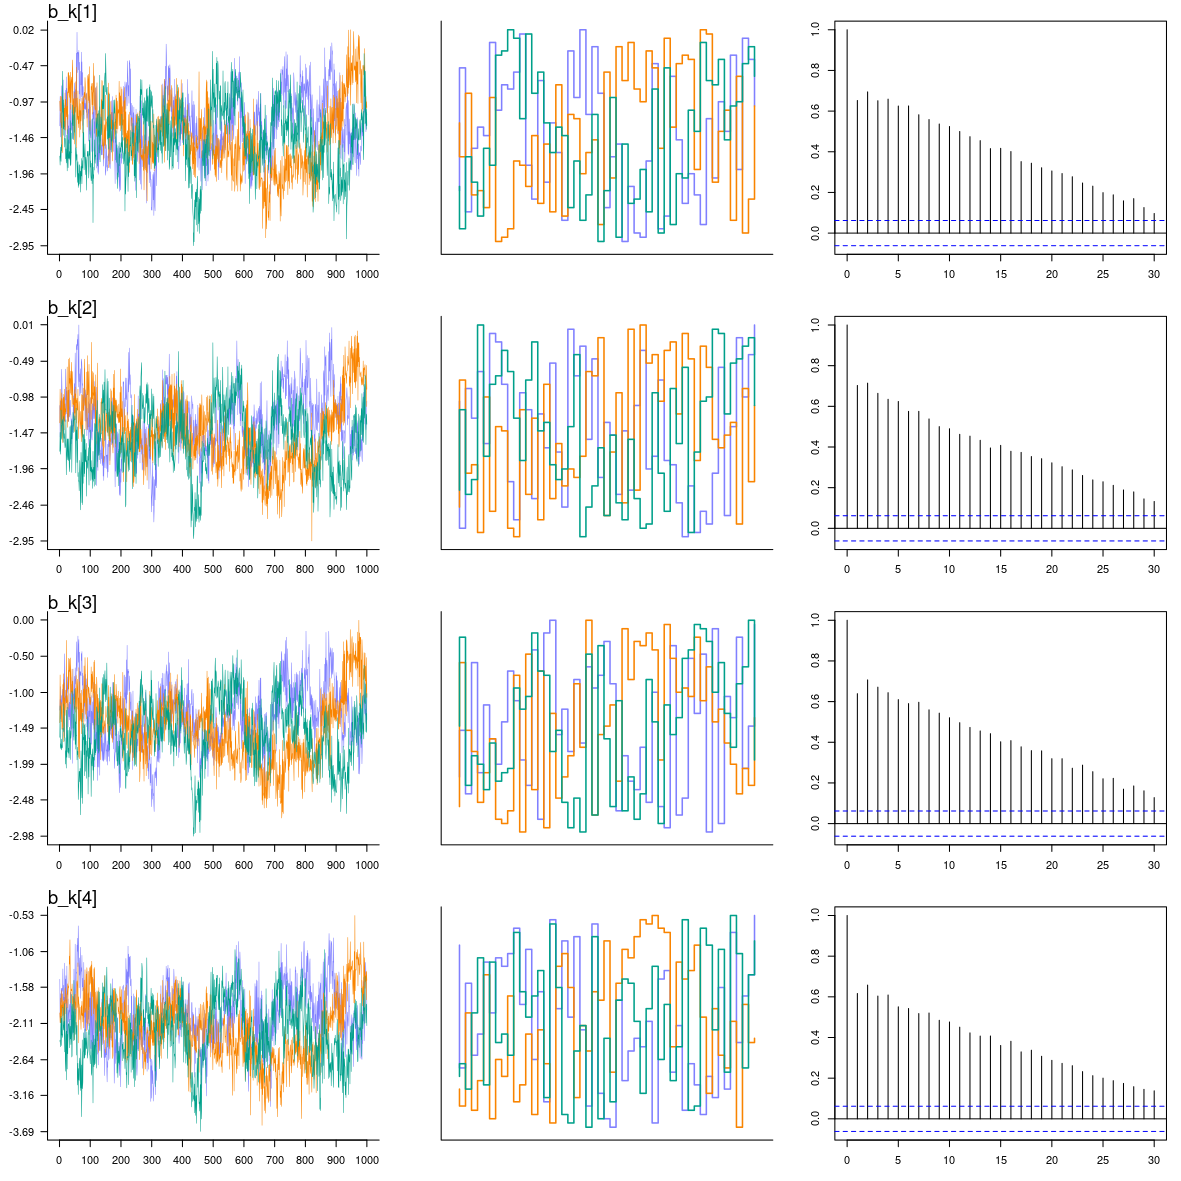
\includegraphics[width=1\linewidth]{FOLV_CE_J100_Ndata1_bk1}
	%
	\caption[First-Order latent variable model (FOLV). Sample size $100$, replica number $1$. Centered parametrization. Difficulty per item. Trace, trank and auto-correlation plots.]%
	{First-Order latent variable model (FOLV). Sample size $100$, replica number $1$. Centered parametrization. Difficulty per item: (Left) trace plot, (Middle) trank plot, (Right) auto-correlation plot.}
	\label{fig:FOLV_CE_chains3}
\end{figure}
%
\begin{figure}[H]
	\centering
	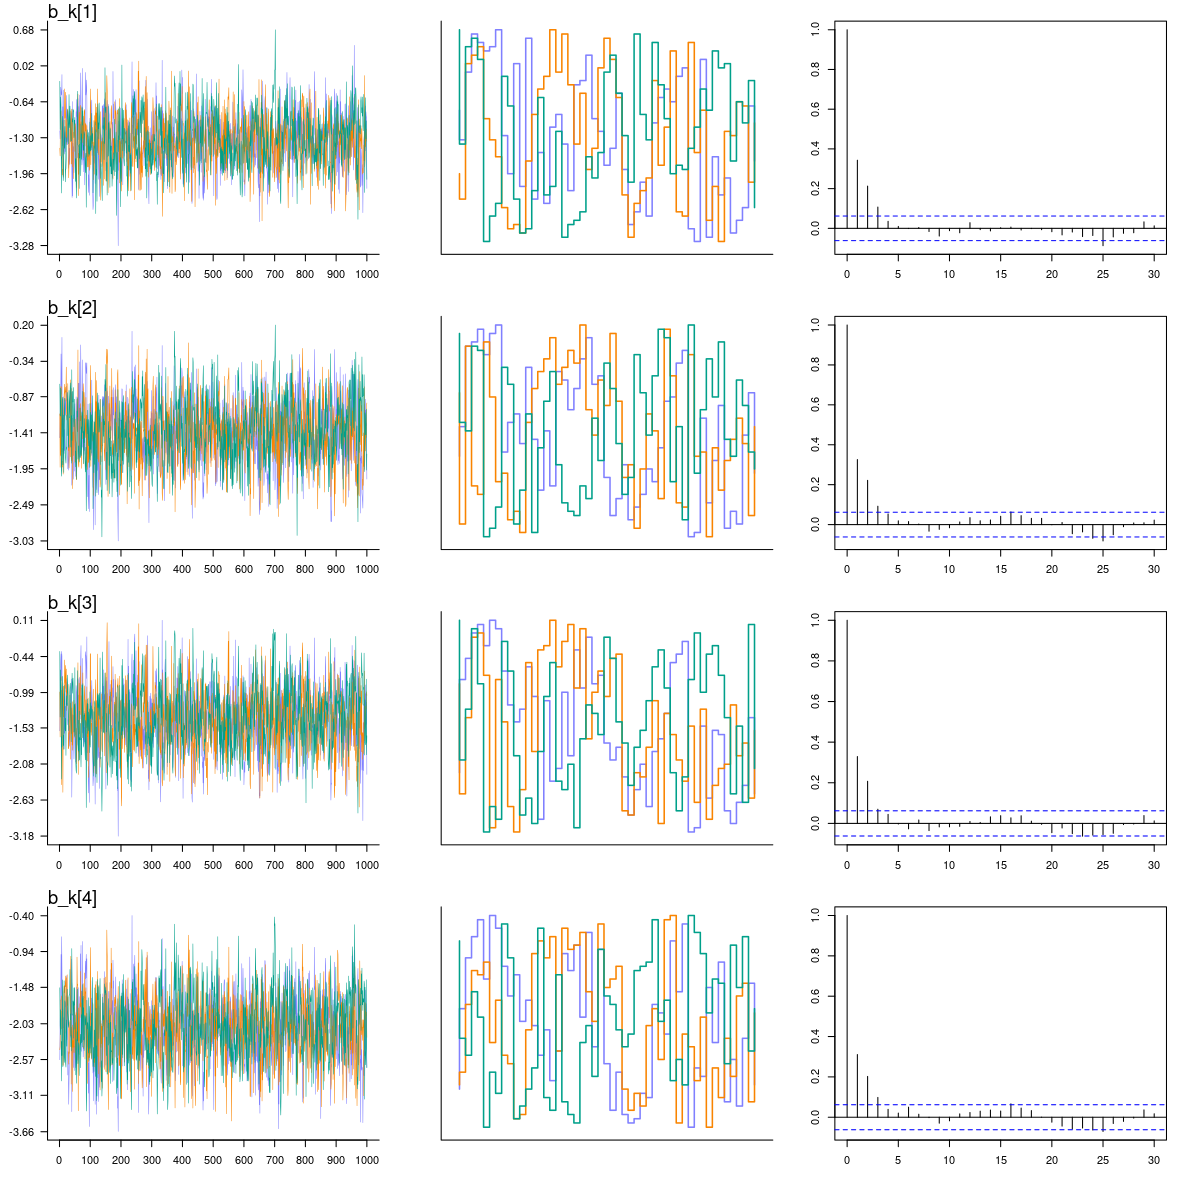
\includegraphics[width=1\linewidth]{FOLV_NC_J100_Ndata1_bk1}
	%
	\caption[First-Order latent variable model (FOLV). Sample size $100$, replica number $1$. Non-centered parametrization. Difficulty per item. Trace, trank and auto-correlation plots.]%
	{First-Order latent variable model (FOLV). Sample size $100$, replica number $1$. Non-centered parametrization. Difficulty per item: (Left) trace plot, (Middle) trank plot, (Right) auto-correlation plot.}
	\label{fig:FOLV_NC_chains3}
\end{figure}
%
\begin{figure}[H]
	\centering
	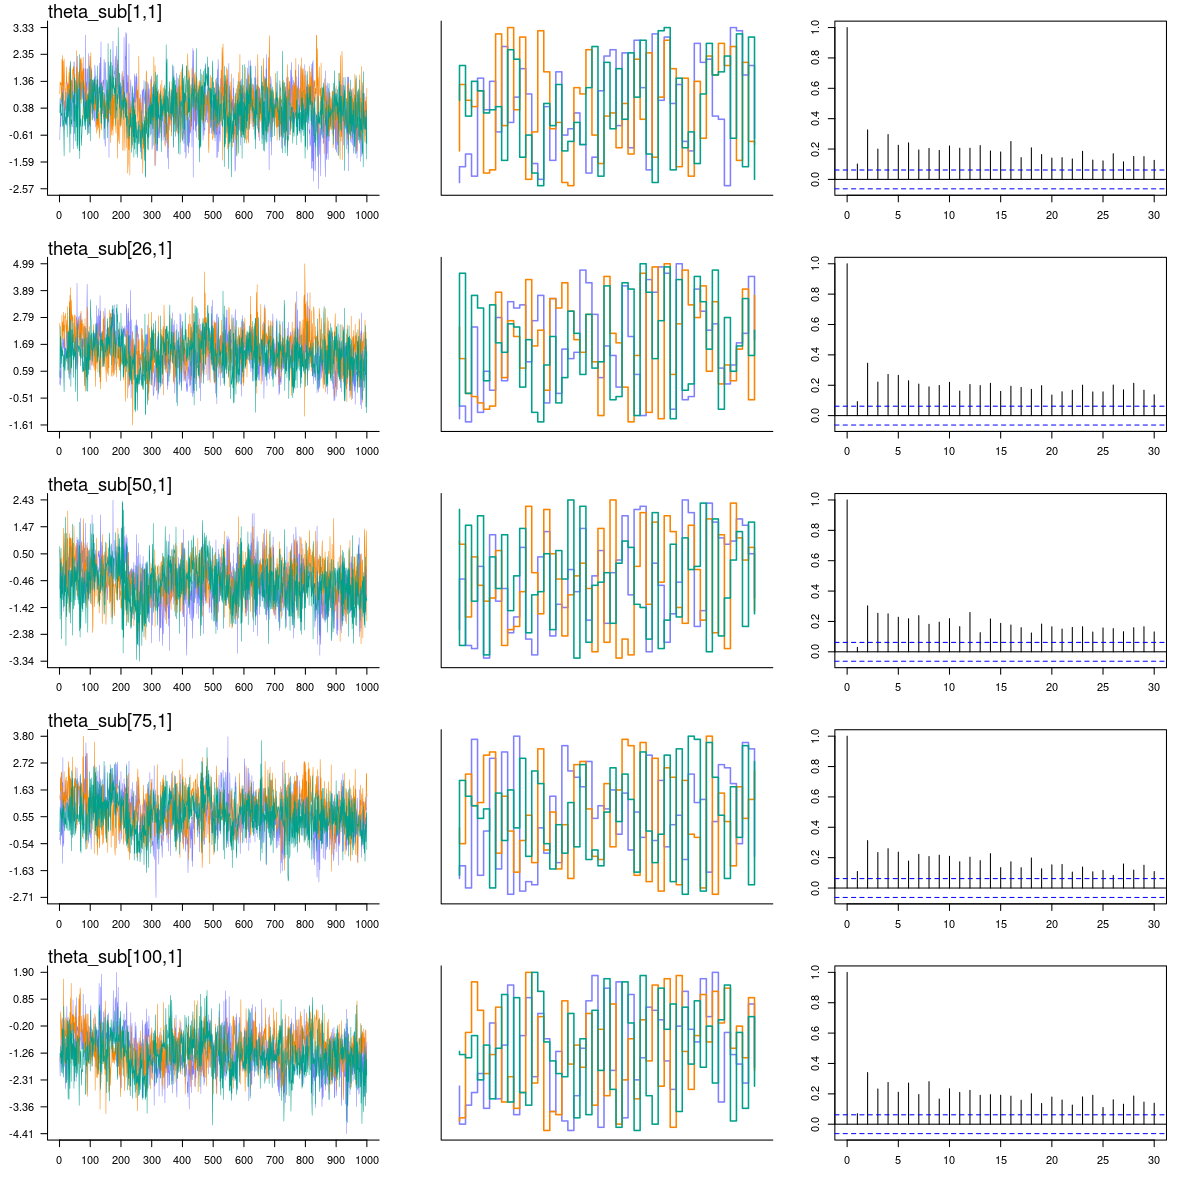
\includegraphics[width=1\linewidth]{FOLV_CE_J100_Ndata6_theta_sub1}
	%
	\caption[First-Order latent variable model (FOLV). Sample size $100$, replica number $6$. Centered parametrization. Individual's first sub-dimension. Trace, trank and auto-correlation plots.]%
	{First-Order latent variable model (FOLV). Sample size $100$, replica number $6$. Centered parametrization. Individual's first sub-dimension: (Left) trace plot, (Middle) trank plot, (Right) auto-correlation plot.}
	\label{fig:FOLV_CE_chains4}
\end{figure}
%
\begin{figure}[H]
	\centering
	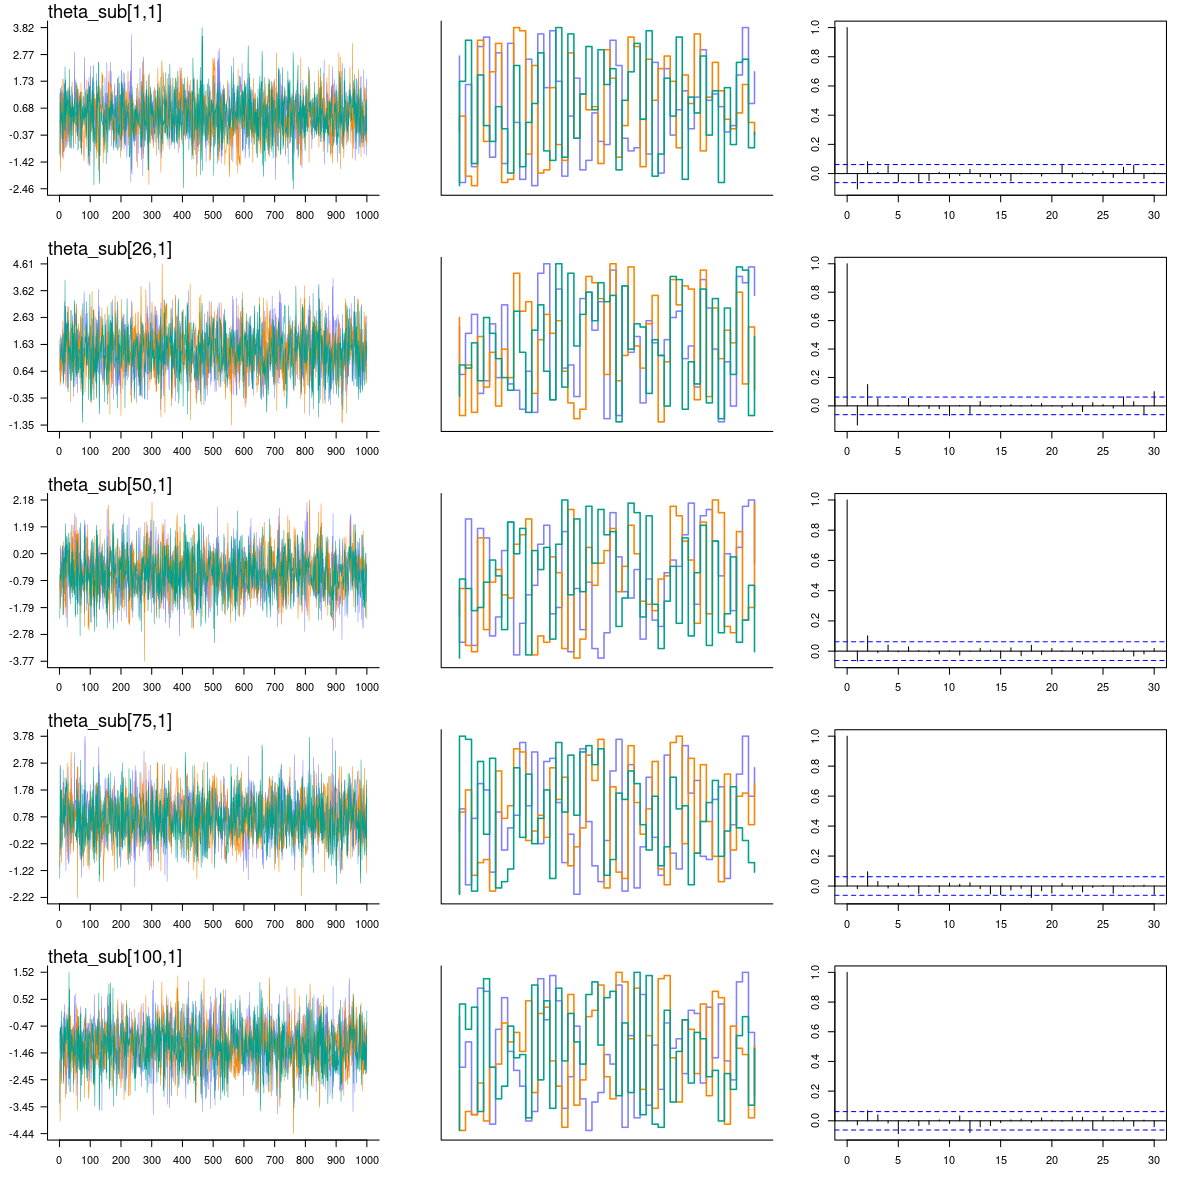
\includegraphics[width=1\linewidth]{FOLV_NC_J100_Ndata6_theta_sub1}
	%
	\caption[First-Order latent variable model (FOLV). Sample size $100$, replica number $6$. Non-centered parametrization. Individual's first sub-dimension. Trace, trank and auto-correlation plots.]%
	{First-Order latent variable model (FOLV). Sample size $100$, replica number $6$. Non-centered parametrization. Individual's first sub-dimension: (Left) trace plot, (Middle) trank plot, (Right) auto-correlation plot.}
	\label{fig:FOLV_NC_chains4}
\end{figure}
%
\begin{figure}[H]
	\centering
	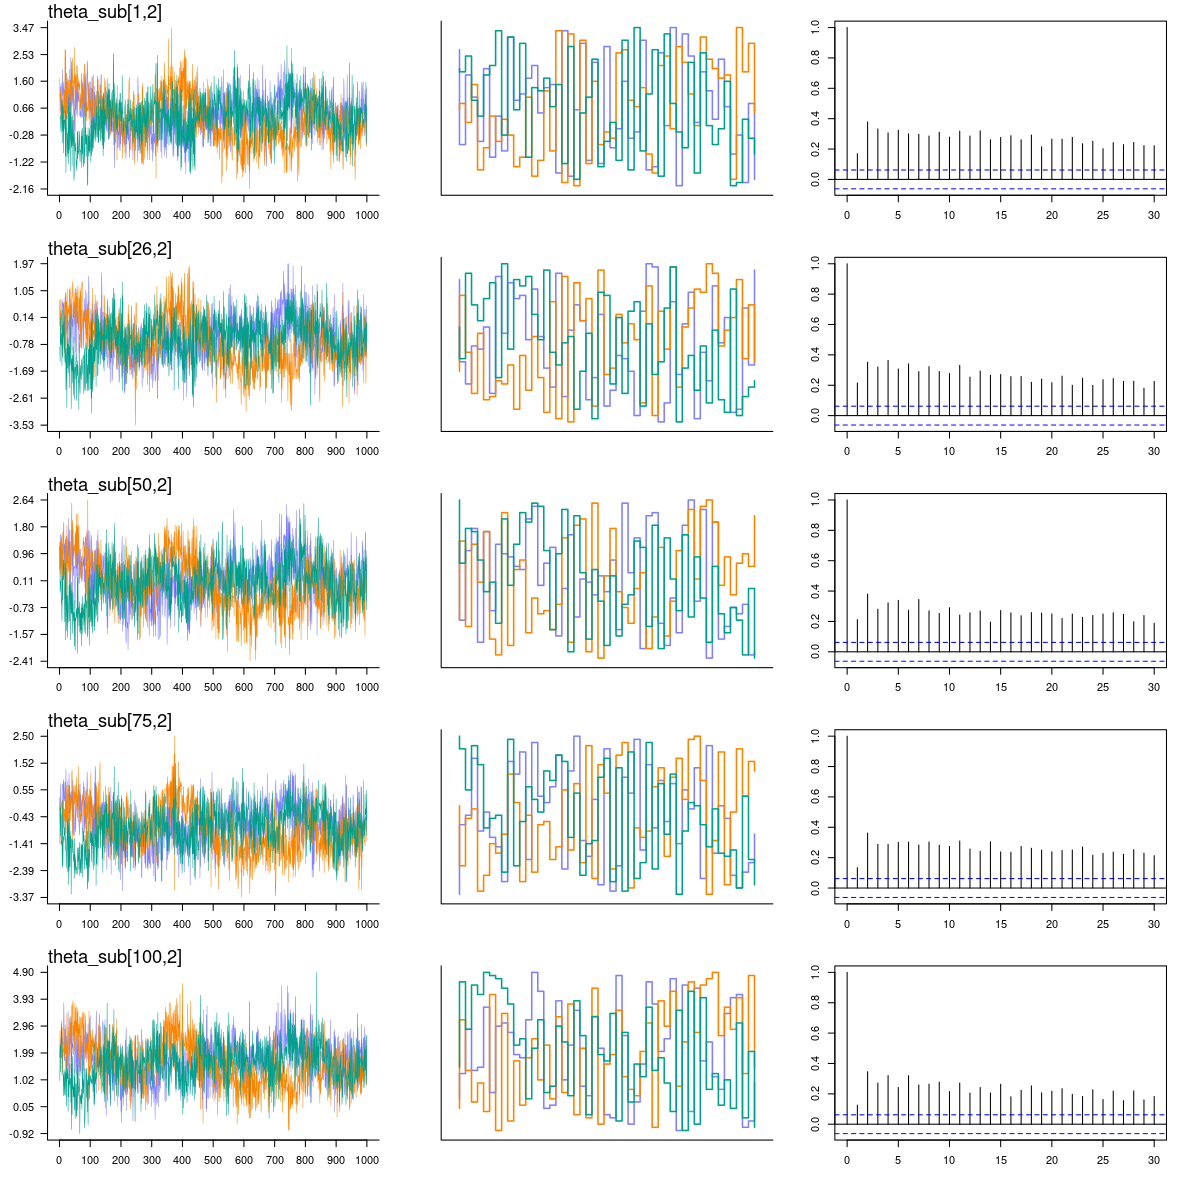
\includegraphics[width=1\linewidth]{FOLV_CE_J100_Ndata7_theta_sub2}
	%
	\caption[First-Order latent variable model (FOLV). Sample size $100$, replica number $7$. Centered parametrization. Individual's second sub-dimension. Trace, trank and auto-correlation plots.]%
	{First-Order latent variable model (FOLV). Sample size $100$, replica number $7$. Centered parametrization. Individual's second sub-dimension: (Left) trace plot, (Middle) trank plot, (Right) auto-correlation plot.}
	\label{fig:FOLV_CE_chains5}
\end{figure}
%
\begin{figure}[H]
	\centering
	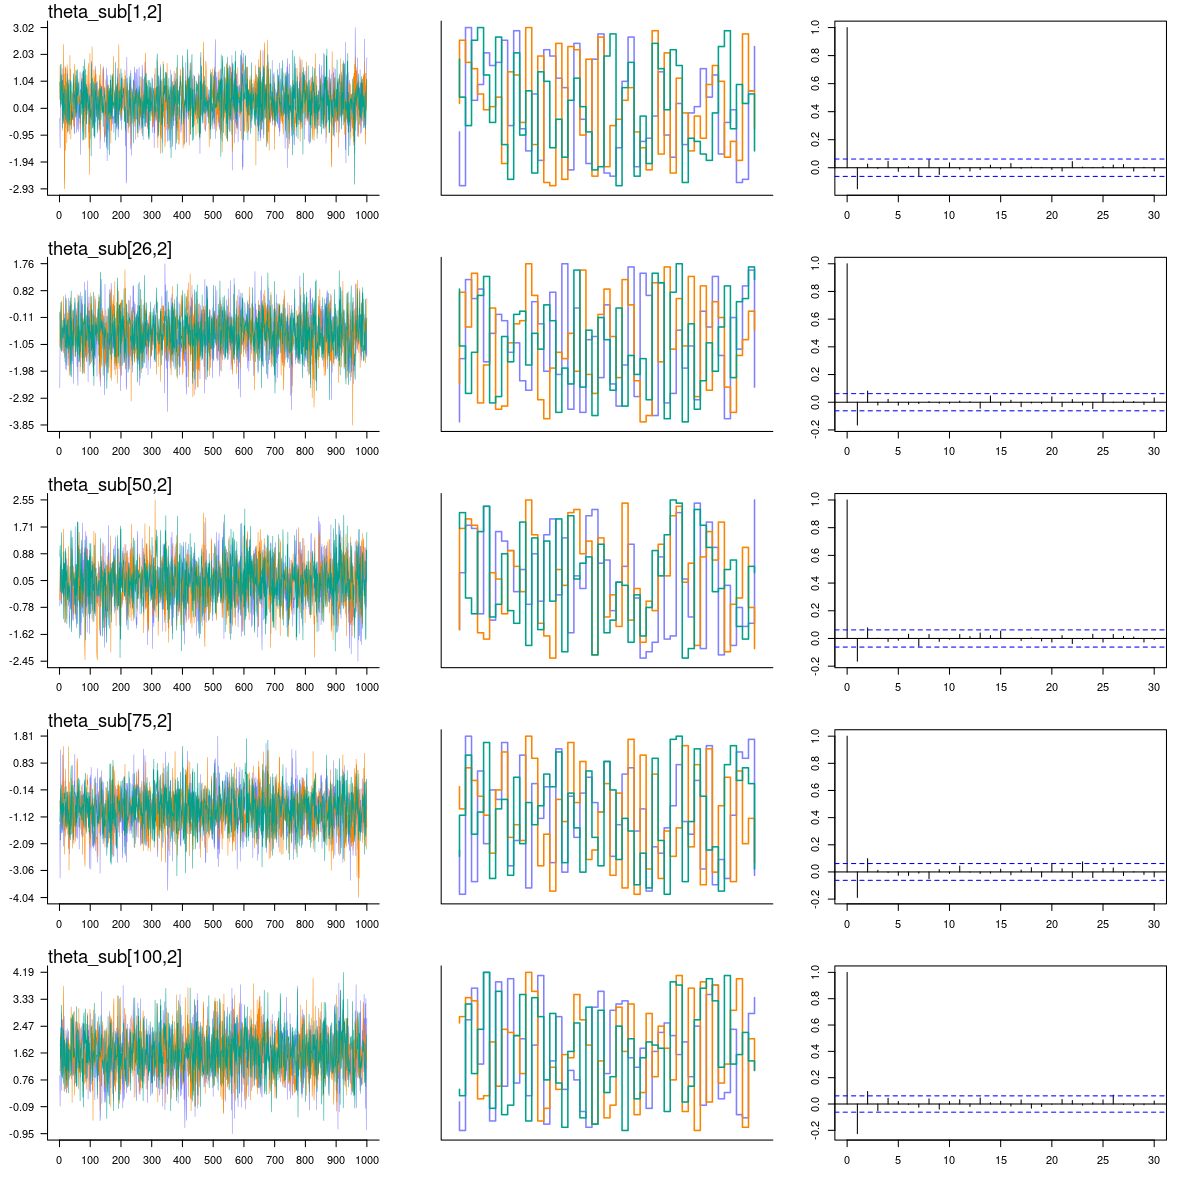
\includegraphics[width=1\linewidth]{FOLV_NC_J100_Ndata7_theta_sub2}
	%
	\caption[First-Order latent variable model (FOLV). Sample size $100$, replica number $7$. Non-centered parametrization. Individual's second sub-dimension. Trace, trank and auto-correlation plots.]%
	{First-Order latent variable model (FOLV). Sample size $100$, replica number $7$. Non-centered parametrization. Individual's second sub-dimension: (Left) trace plot, (Middle) trank plot, (Right) auto-correlation plot.}
	\label{fig:FOLV_NC_chains5}
\end{figure}
%
\begin{figure}[H]
	\centering
	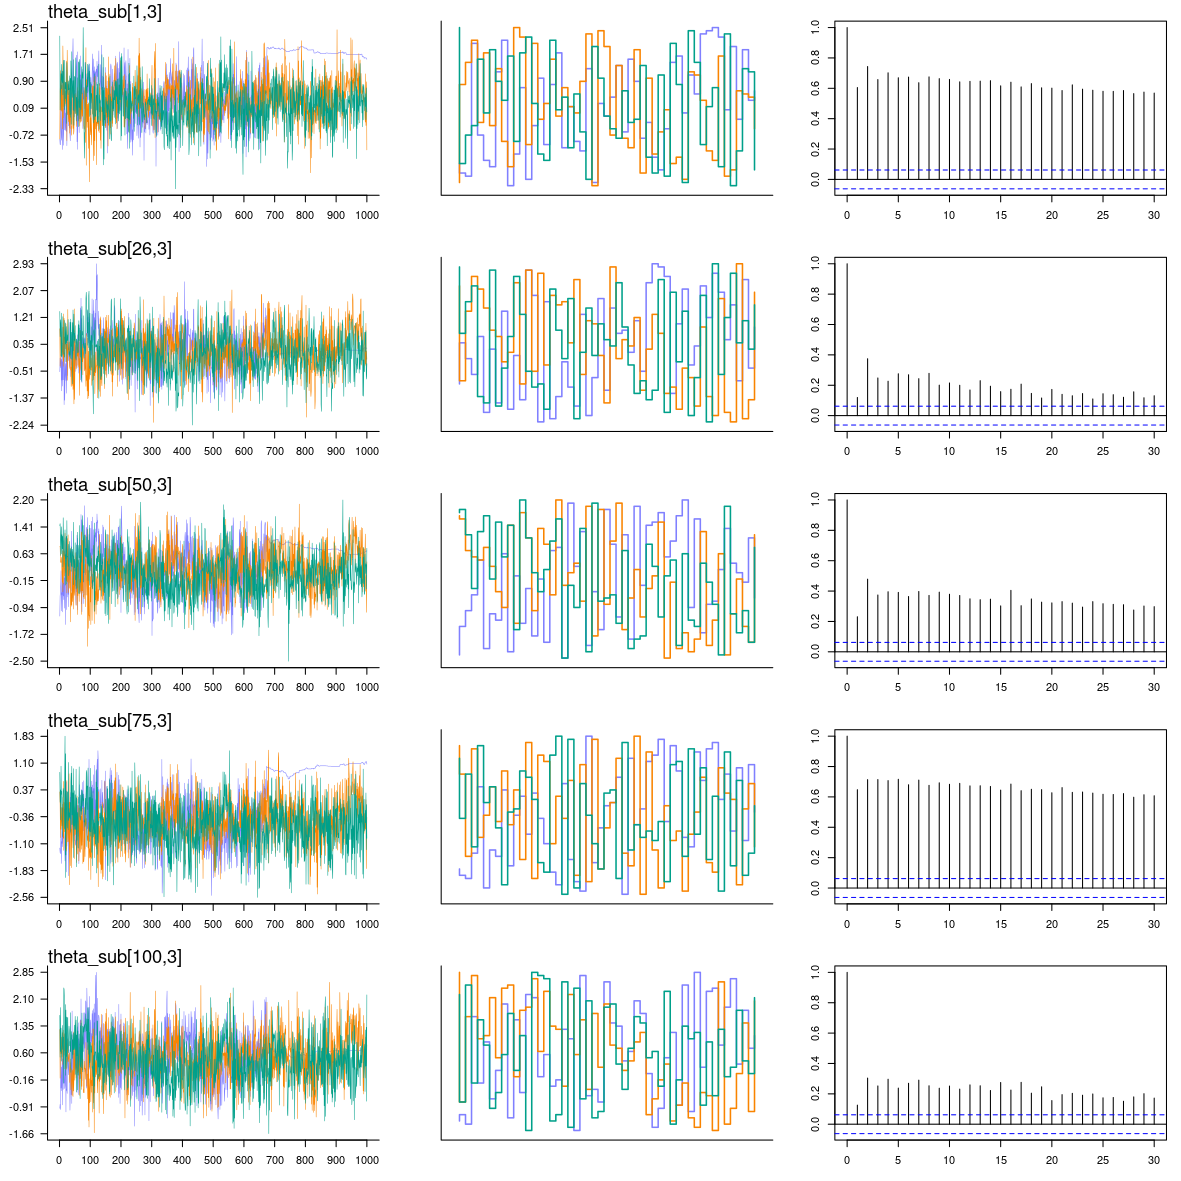
\includegraphics[width=1\linewidth]{FOLV_CE_J100_Ndata8_theta_sub3}
	%
	\caption[First-Order latent variable model (FOLV). Sample size $100$, replica number $8$. Centered parametrization. Individual's third sub-dimension. Trace, trank and auto-correlation plots.]%
	{First-Order latent variable model (FOLV). Sample size $100$, replica number $8$. Centered parametrization. Individual's third sub-dimension: (Left) trace plot, (Middle) trank plot, (Right) auto-correlation plot.}
	\label{fig:FOLV_CE_chains6}
\end{figure}
%
\begin{figure}[H]
	\centering
	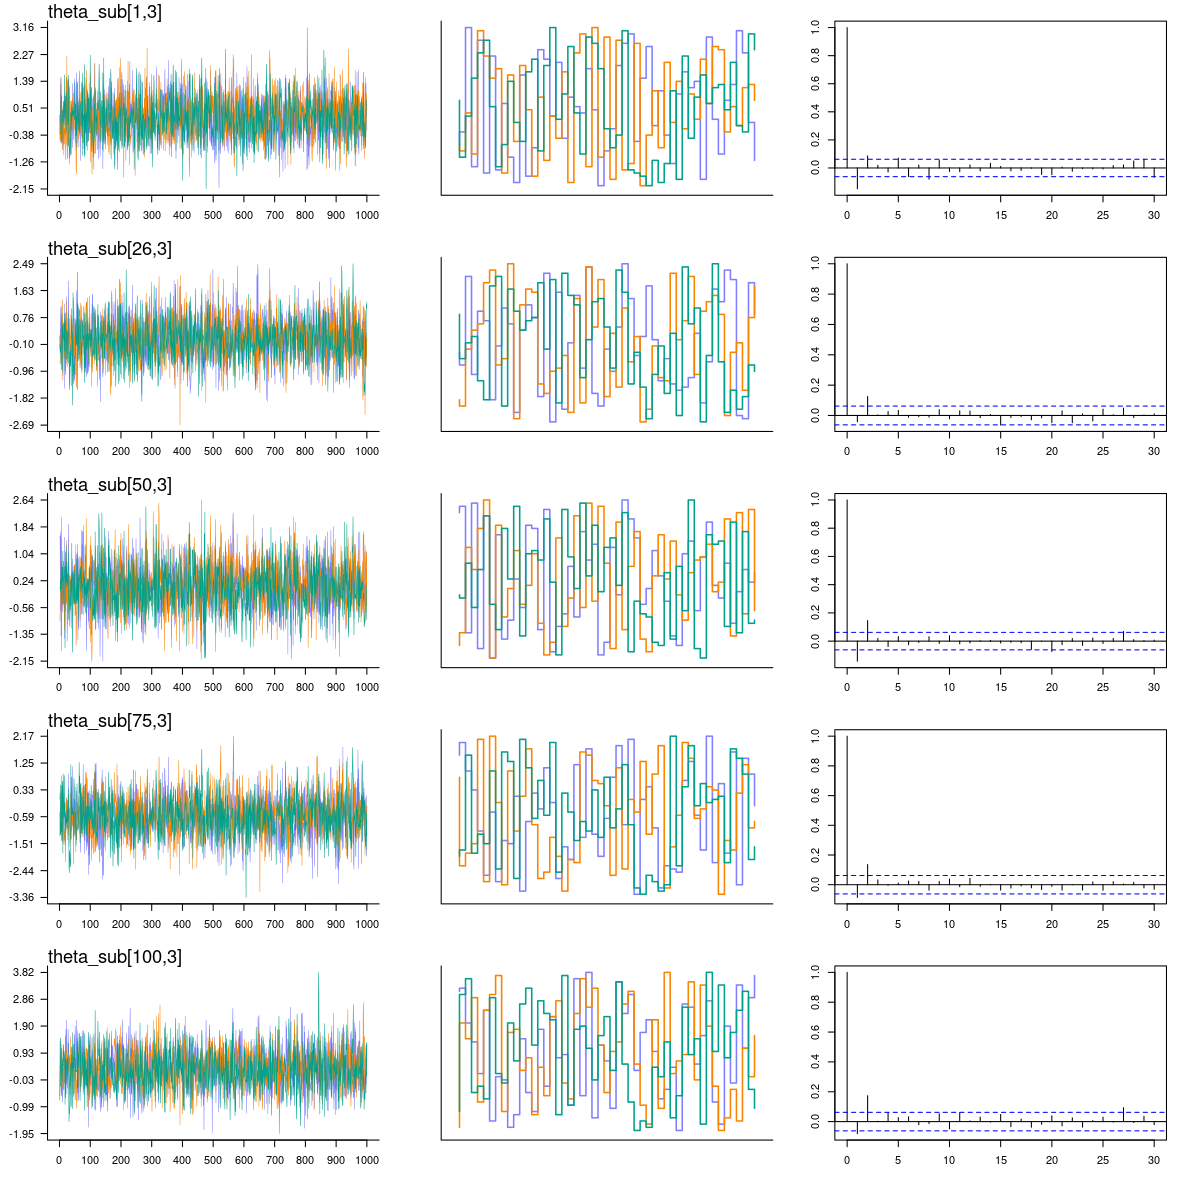
\includegraphics[width=1\linewidth]{FOLV_NC_J100_Ndata8_theta_sub3}
	%
	\caption[First-Order latent variable model (FOLV). Sample size $100$, replica number $8$. Non-centered parametrization. Individual's third sub-dimension. Trace, trank and auto-correlation plots.]%
	{First-Order latent variable model (FOLV). Sample size $100$, replica number $8$. Non-centered parametrization. Individual's third sub-dimension: (Left) trace plot, (Middle) trank plot, (Right) auto-correlation plot.}
	\label{fig:FOLV_NC_chains6}
\end{figure}
%
\begin{figure}[H]
	\centering
	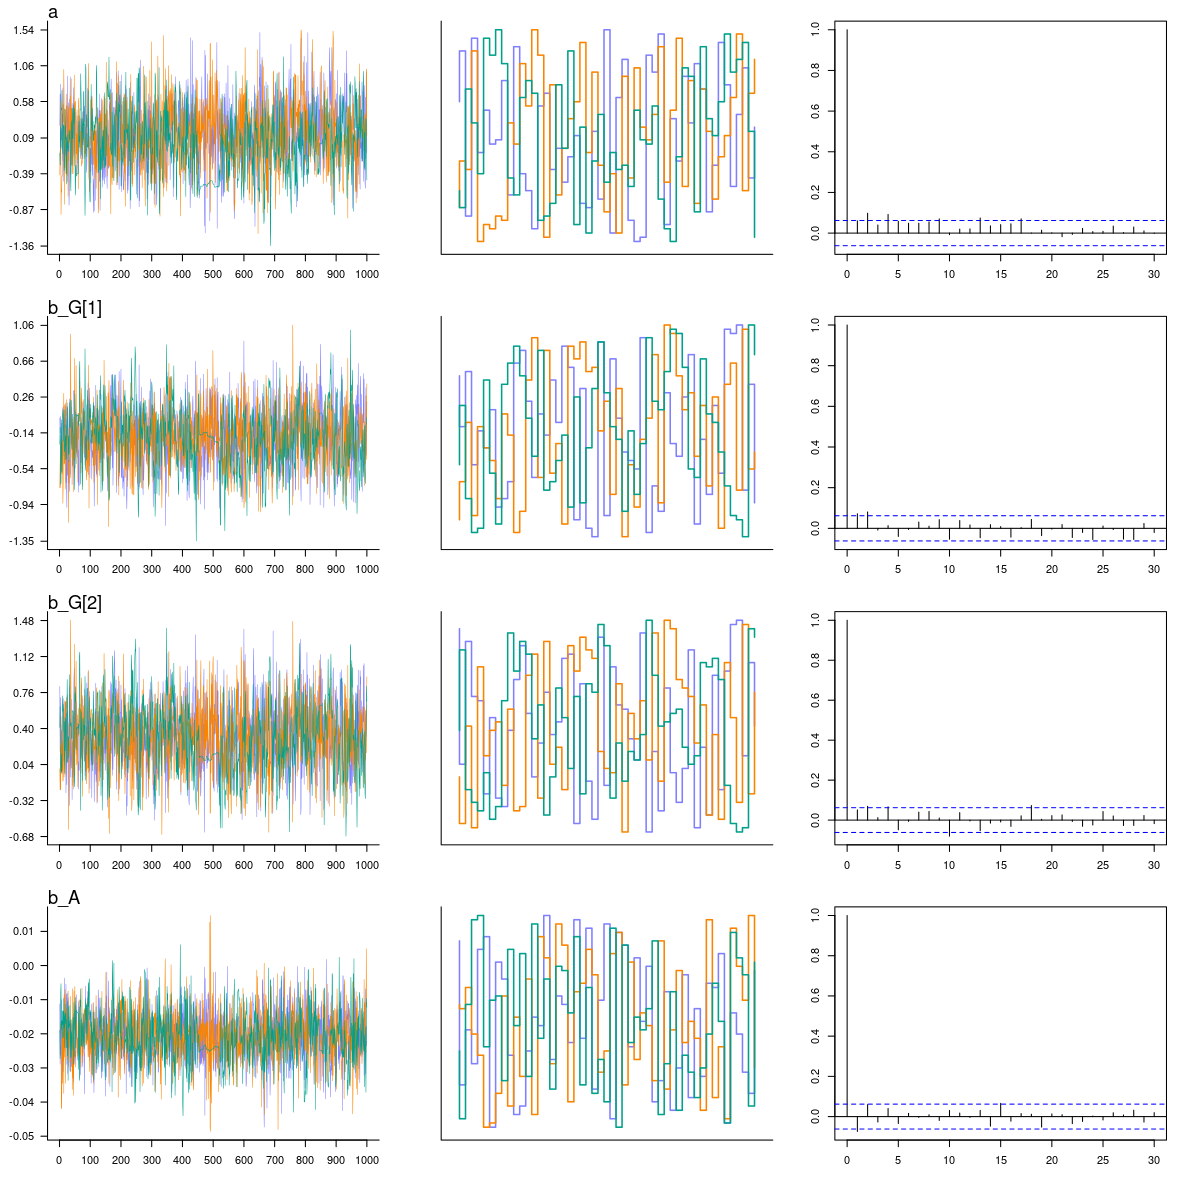
\includegraphics[width=1\linewidth]{FOLV_CE_J100_Ndata4_reg1}
	%
	\caption[First-Order latent variable model (FOLV). Sample size $100$, replica number $4$. Centered parametrization. Regression parameters. Trace, trank and auto-correlation plots.]%
	{First-Order latent variable model (FOLV). Sample size $100$, replica number $4$. Centered parametrization. Regression parameters: (Left) trace plot, (Middle) trank plot, (Right) auto-correlation plot.}
	\label{fig:FOLV_CE_chains7}
\end{figure}
%
\begin{figure}[H]
	\centering
	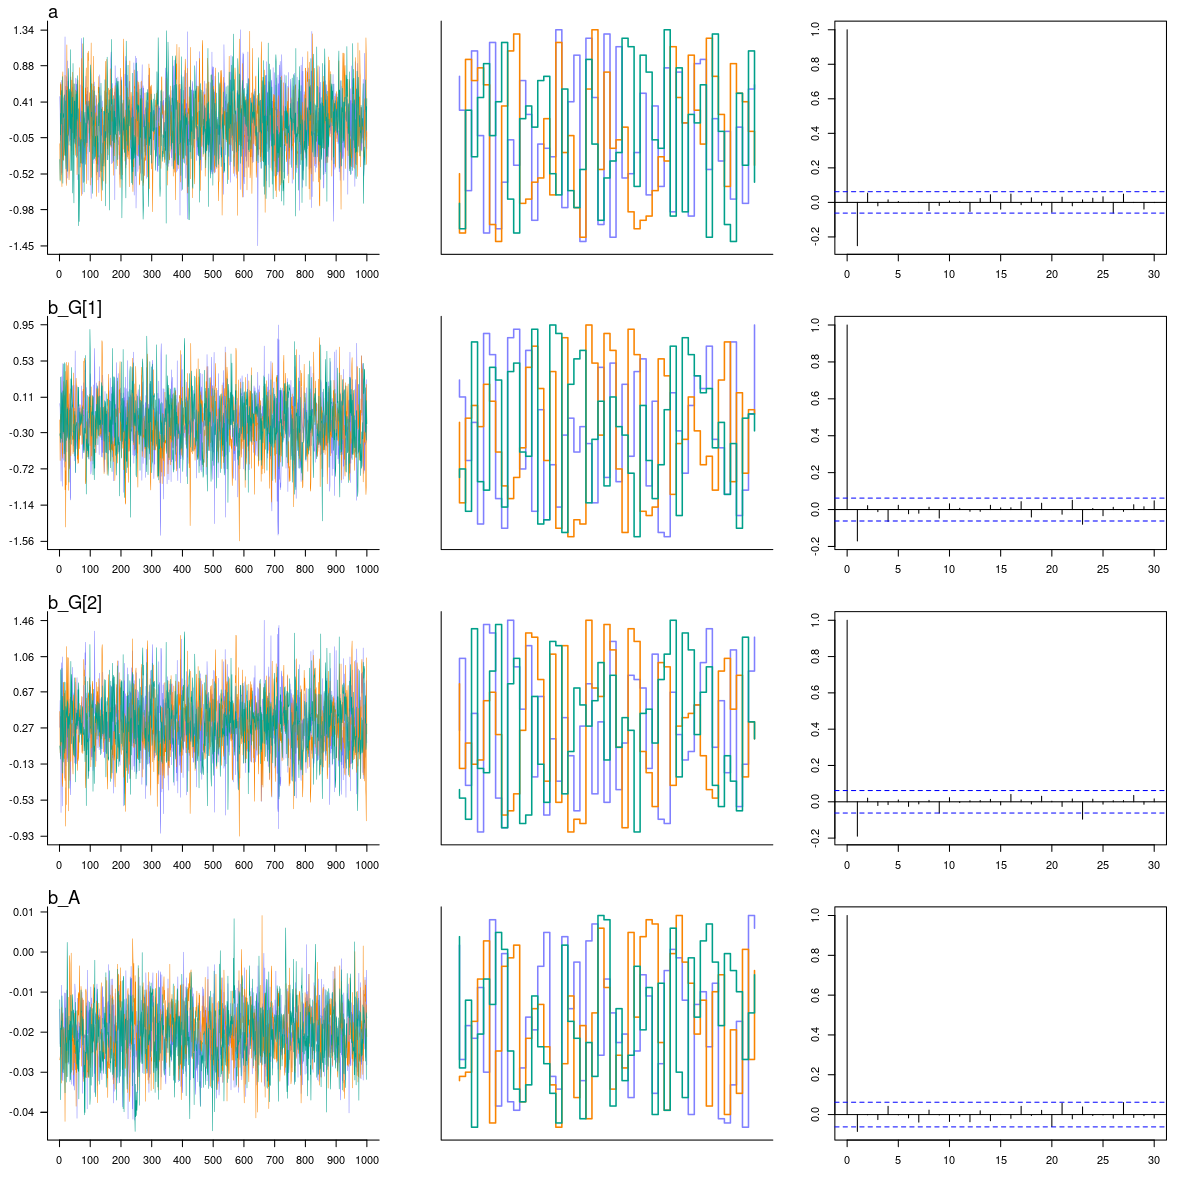
\includegraphics[width=1\linewidth]{FOLV_NC_J100_Ndata4_reg1}
	%
	\caption[First-Order latent variable model (FOLV). Sample size $100$, replica number $4$. Non-centered parametrization. Regression parameters. Trace, trank and auto-correlation plots.]%
	{First-Order latent variable model (FOLV). Sample size $100$, replica number $4$. Non-centered parametrization. Regression parameters: (Left) trace plot, (Middle) trank plot, (Right) auto-correlation plot.}
	\label{fig:FOLV_NC_chains7}
\end{figure}
%
\begin{figure}[H]
	\centering
	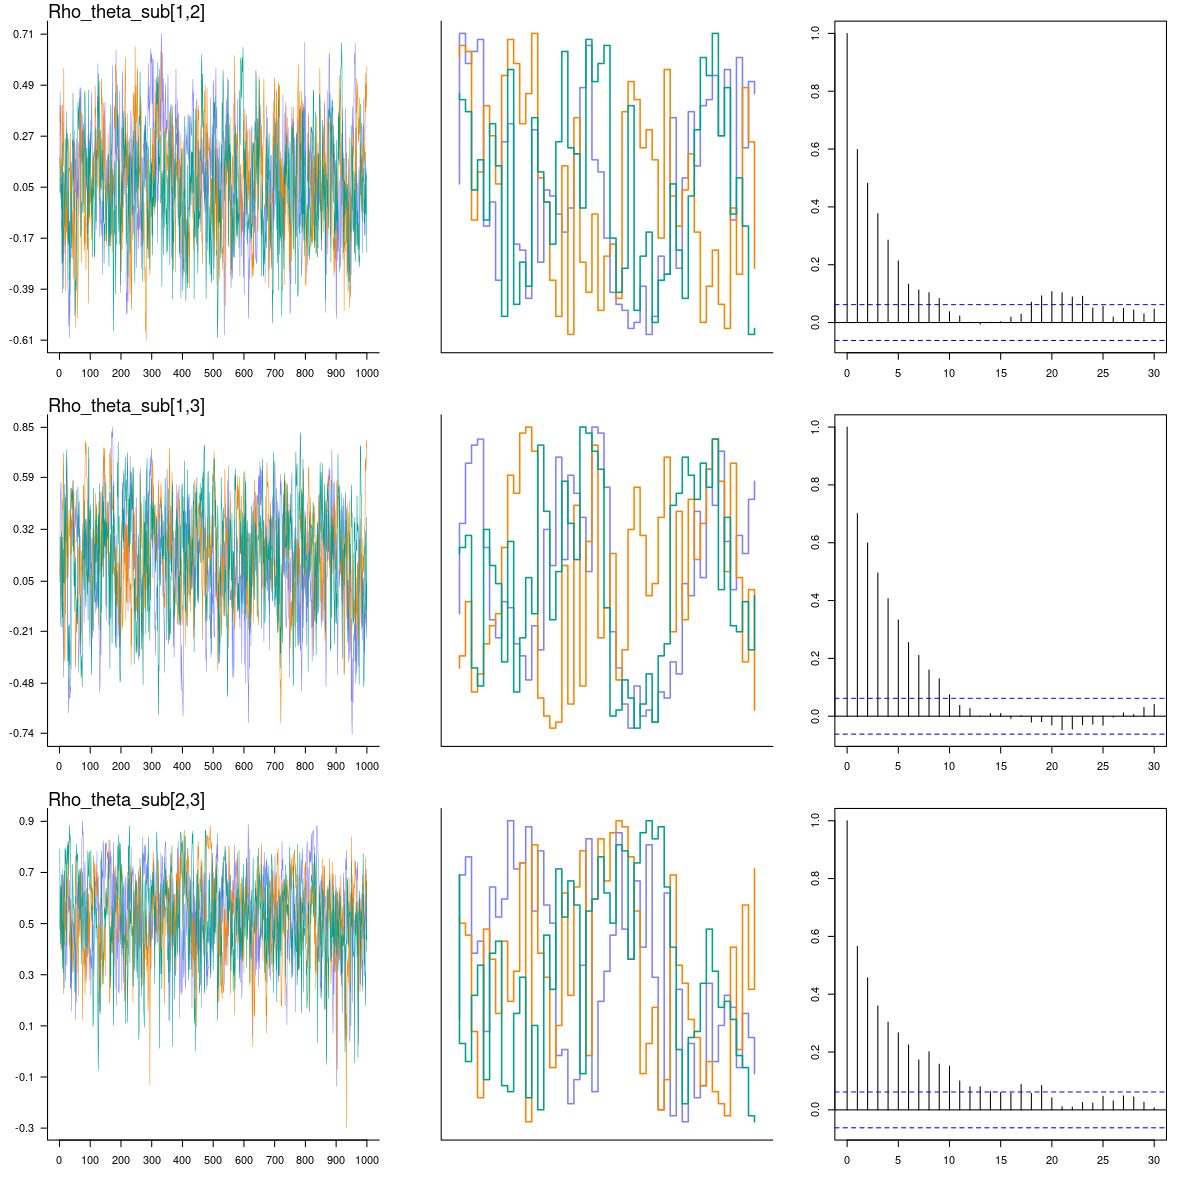
\includegraphics[width=1\linewidth]{FOLV_CE_J100_Ndata5_Rho}
	%
	\caption[First-Order latent variable model (FOLV). Sample size $100$, replica number $5$. Centered parametrization. Correlation of sub-dimensions. Trace, trank and auto-correlation plots.]%
	{First-Order latent variable model (FOLV). Sample size $100$, replica number $5$. Centered parametrization. Correlation of sub-dimensions: (Left) trace plot, (Middle) trank plot, (Right) auto-correlation plot.}
	\label{fig:FOLV_CE_chains8}
\end{figure}
%
\begin{figure}[H]
	\centering
	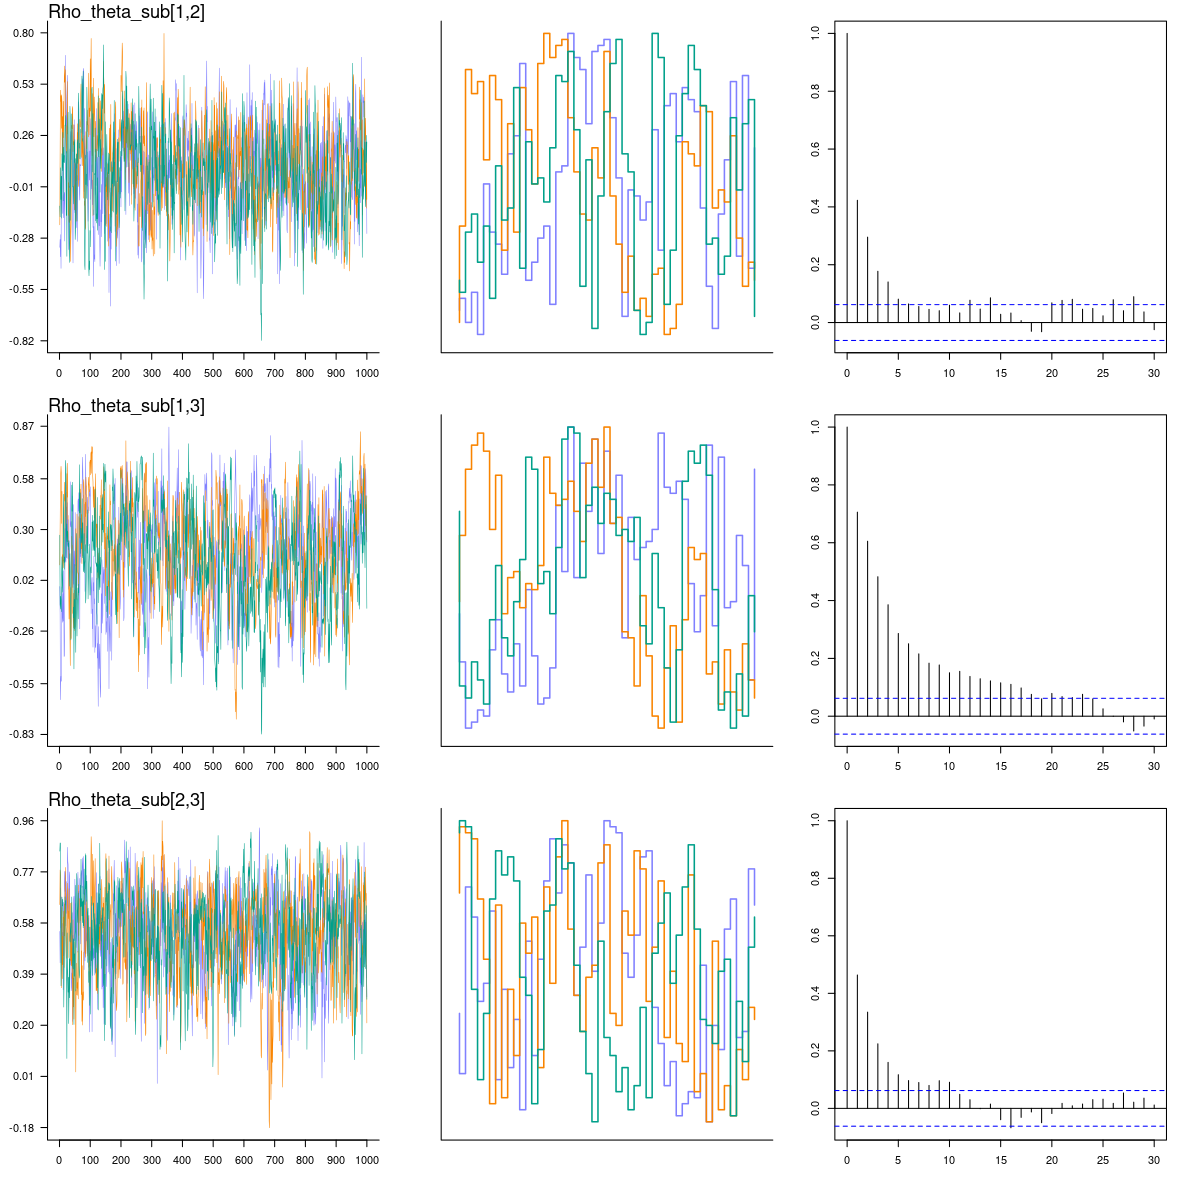
\includegraphics[width=1\linewidth]{FOLV_NC_J100_Ndata5_Rho}
	%
	\caption[First-Order latent variable model (FOLV). Sample size $100$, replica number $5$. Non-centered parametrization. Correlation of sub-dimensions. Trace, trank and auto-correlation plots.]%
	{First-Order latent variable model (FOLV). Sample size $100$, replica number $5$. Non-centered parametrization. Correlation of sub-dimensions: (Left) trace plot, (Middle) trank plot, (Right) auto-correlation plot.}
	\label{fig:FOLV_NC_chains8}
\end{figure}
%
\begin{figure}[H]
	\centering
	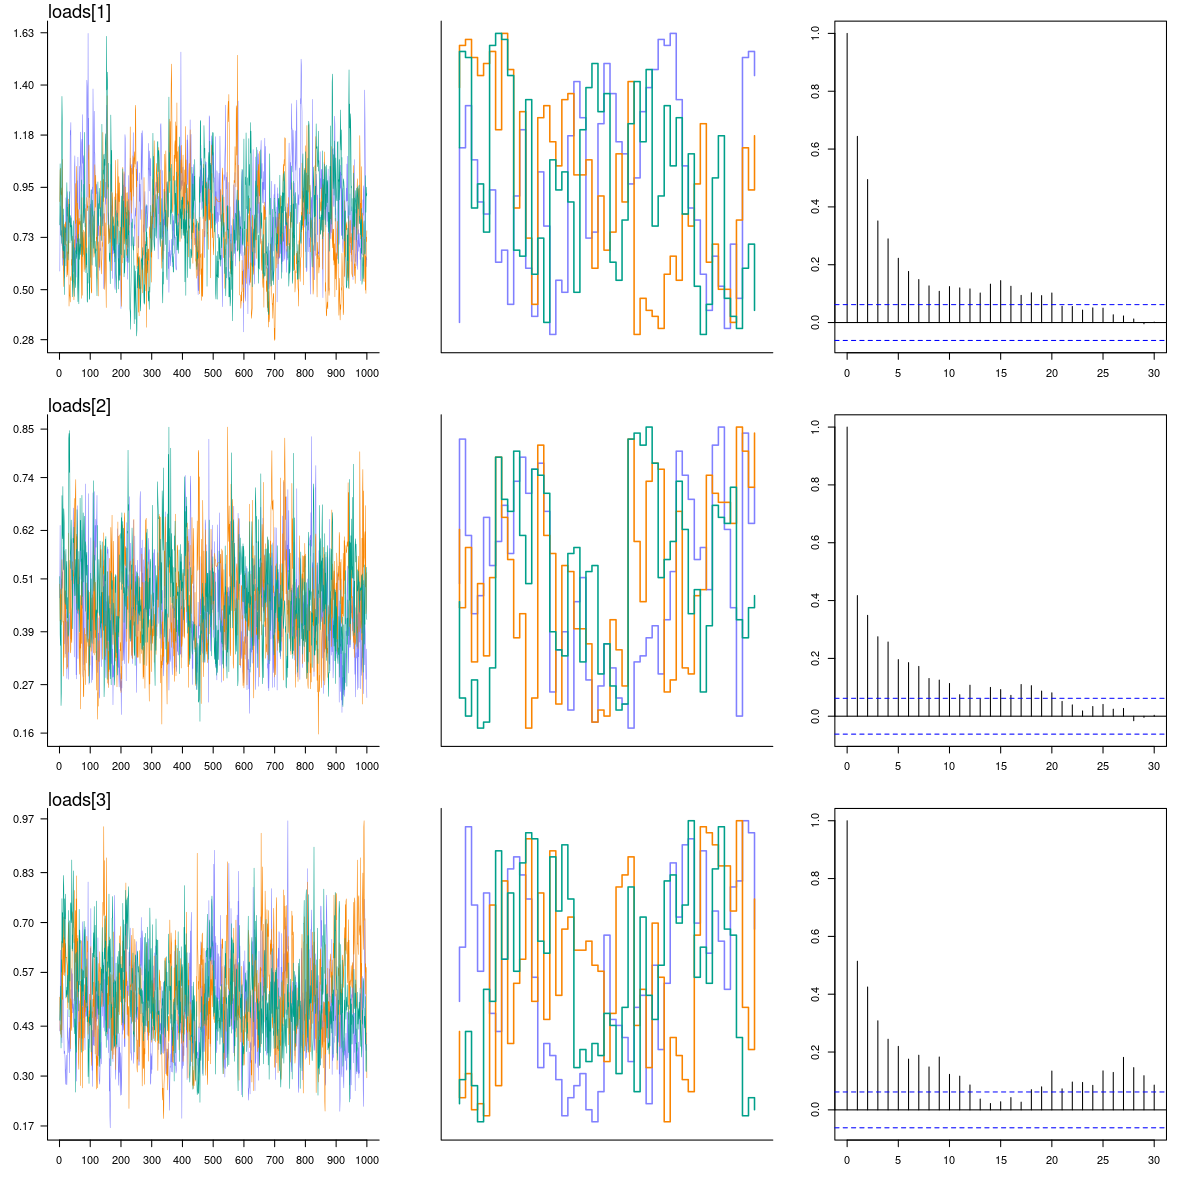
\includegraphics[width=1\linewidth]{SOLV_CE_J100_Ndata9_loads}
	%
	\caption[Second-Order latent variable model (SOLV). Sample size $100$, replica number $9$. Centered parametrization. Loadings. Trace, trank and auto-correlation plots.]%
	{Second-Order latent variable model (SOLV). Sample size $100$, replica number $9$. Centered parametrization. Loadings: (Left) trace plot, (Middle) trank plot, (Right) auto-correlation plot.}
	\label{fig:SOLV_CE_chains1}
\end{figure}
%
\begin{figure}[H]
	\centering
	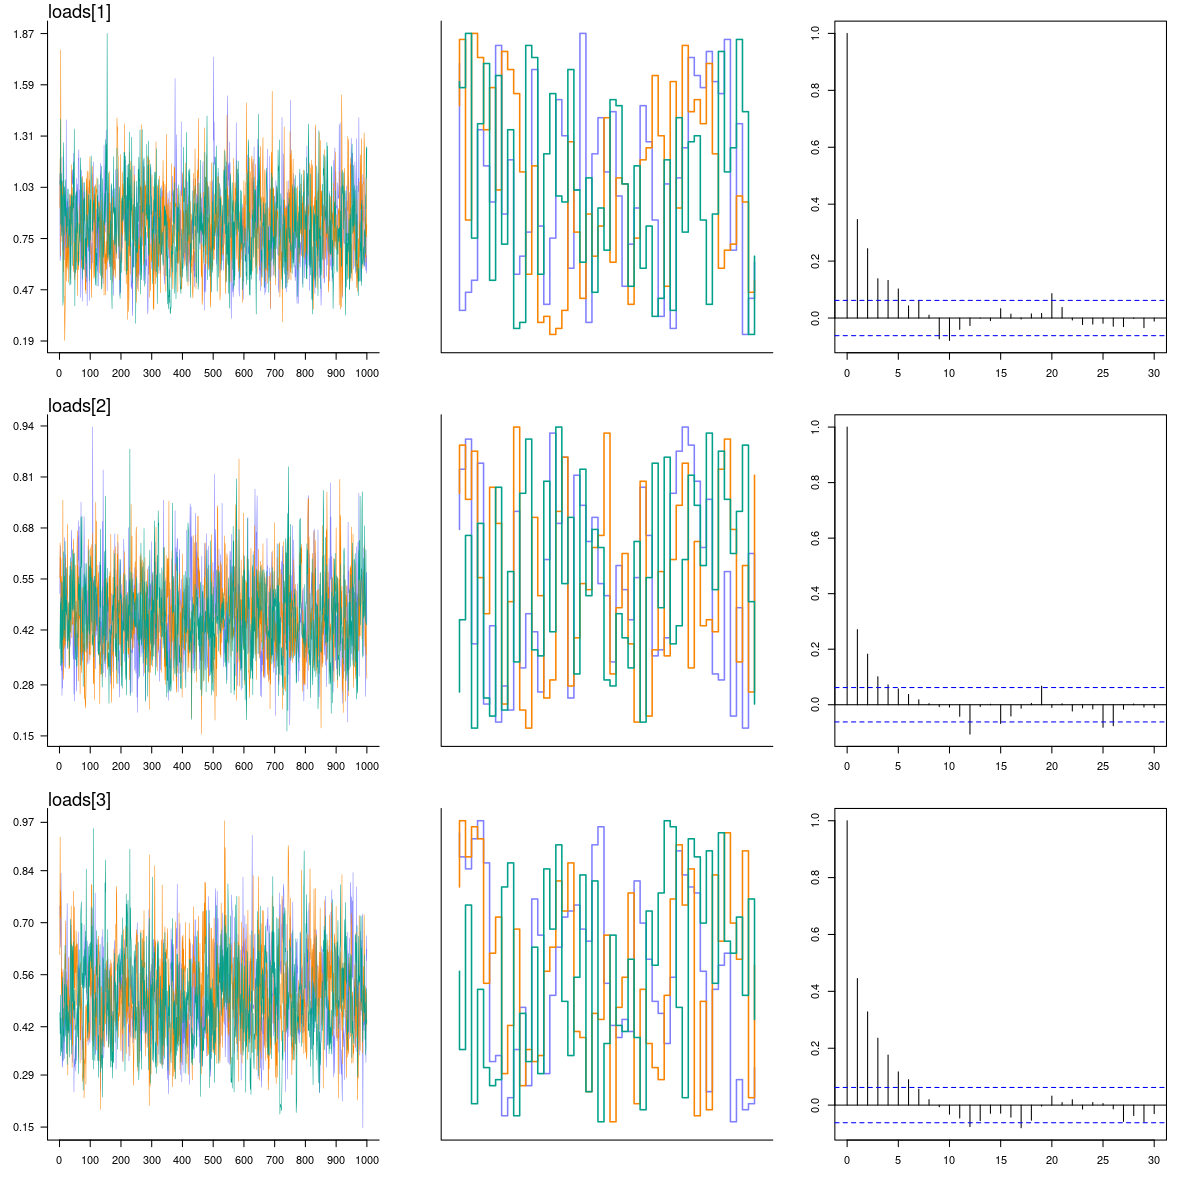
\includegraphics[width=1\linewidth]{SOLV_NC_J100_Ndata9_loads}
	%
	\caption[Second-Order latent variable model (SOLV). Sample size $100$, replica number $9$. Non-centered parametrization. Loadings. Trace, trank and auto-correlation plots.]%
	{Second-Order latent variable model (SOLV). Sample size $100$, replica number $9$. Non-centered parametrization. Loadings: (Left) trace plot, (Middle) trank plot, (Right) auto-correlation plot.}
	\label{fig:SOLV_NC_chains1}
\end{figure}
%
\begin{figure}[H]
	\centering
	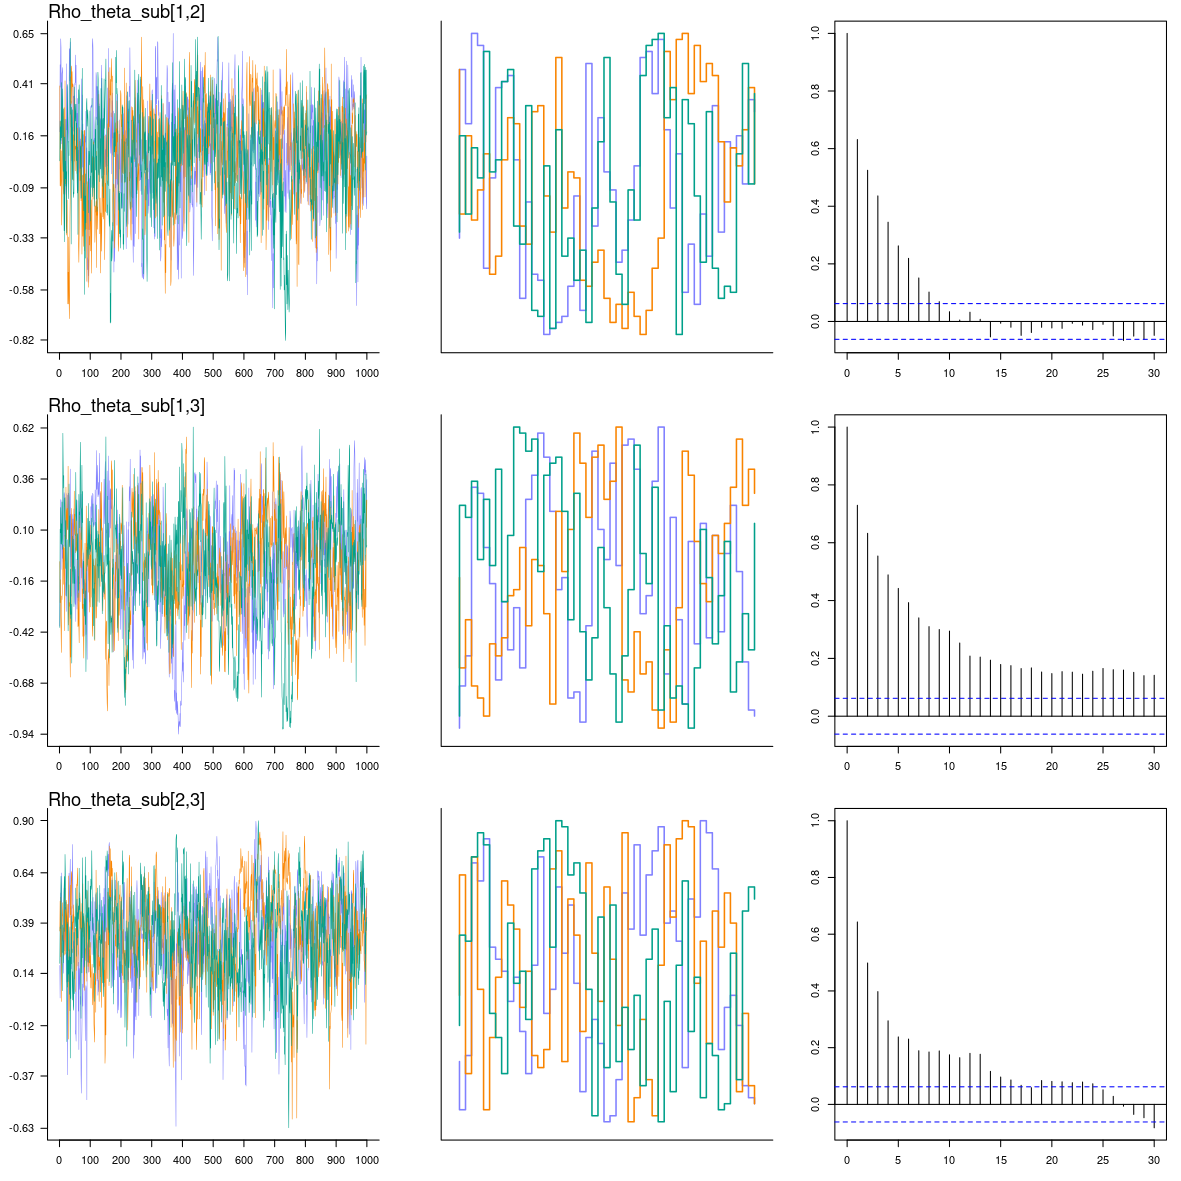
\includegraphics[width=1\linewidth]{SOLV_CE_J100_Ndata1_Rho}
	%
	\caption[Second-Order latent variable model (SOLV). Sample size $100$, replica number $1$. Centered parametrization. Correlation of sub-dimensions. Trace, trank and auto-correlation plots.]%
	{Second-Order latent variable model (SOLV). Sample size $100$, replica number $1$. Centered parametrization. Correlation of sub-dimensions: (Left) trace plot, (Middle) trank plot, (Right) auto-correlation plot.}
	\label{fig:SOLV_CE_chains2}
\end{figure}
%
\begin{figure}[H]
	\centering
	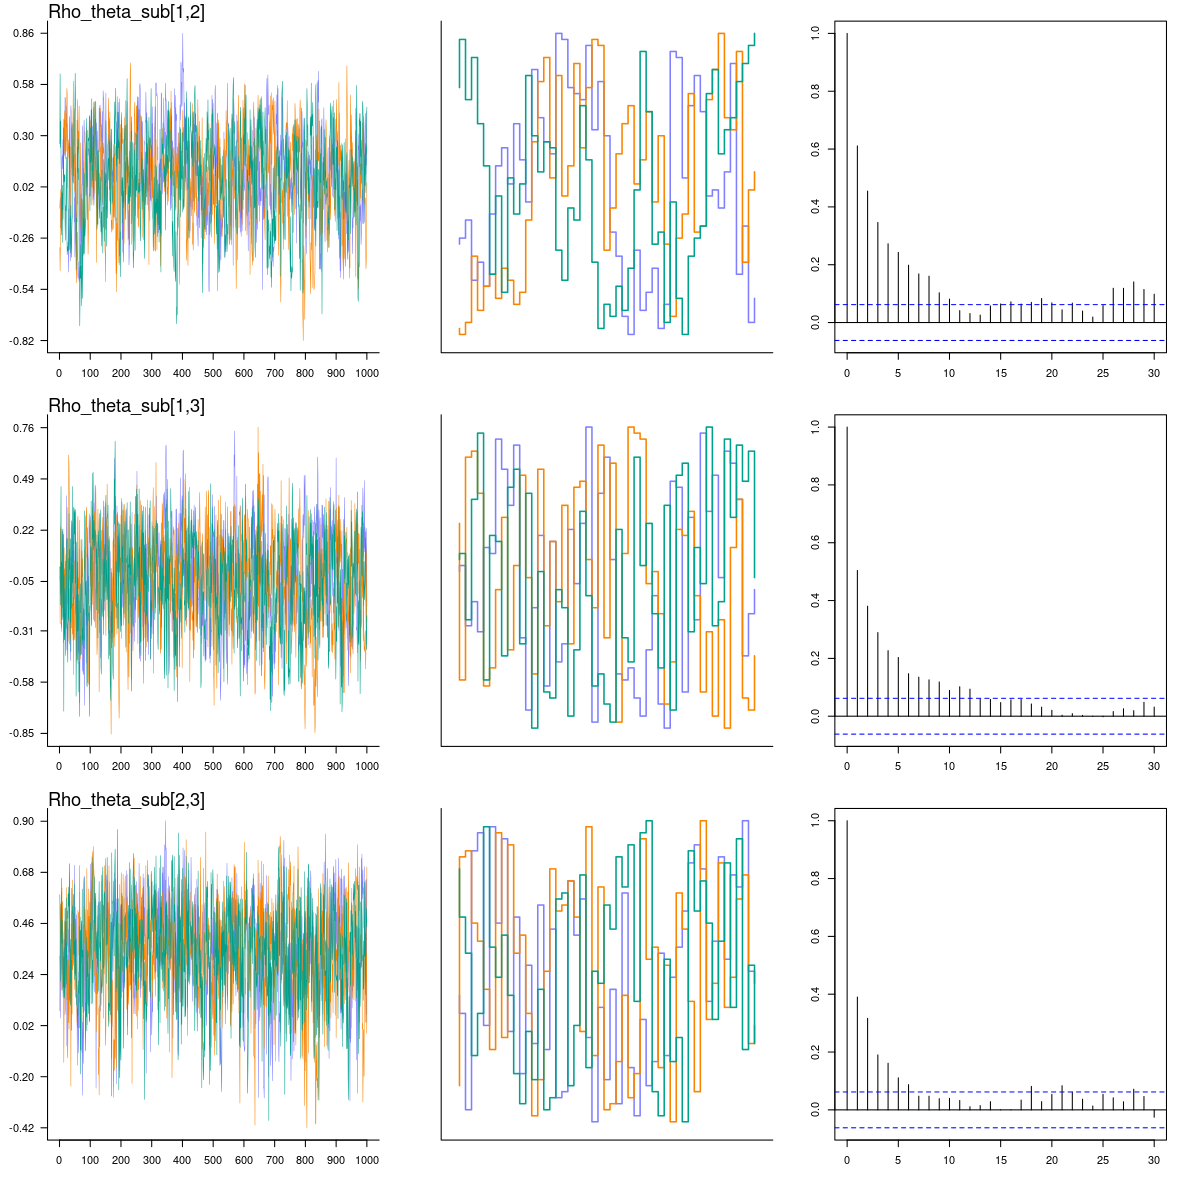
\includegraphics[width=1\linewidth]{SOLV_NC_J100_Ndata1_Rho}
	%
	\caption[Second-Order latent variable model (SOLV). Sample size $100$, replica number $1$. Non-centered parametrization. Correlation of sub-dimensions. Trace, trank and auto-correlation plots.]%
	{Second-Order latent variable model (SOLV). Sample size $100$, replica number $1$. Non-centered parametrization. Correlation of sub-dimensions: (Left) trace plot, (Middle) trank plot, (Right) auto-correlation plot.}
	\label{fig:SOLV_NC_chains2}
\end{figure}
%
\begin{figure}[H]
	\centering
	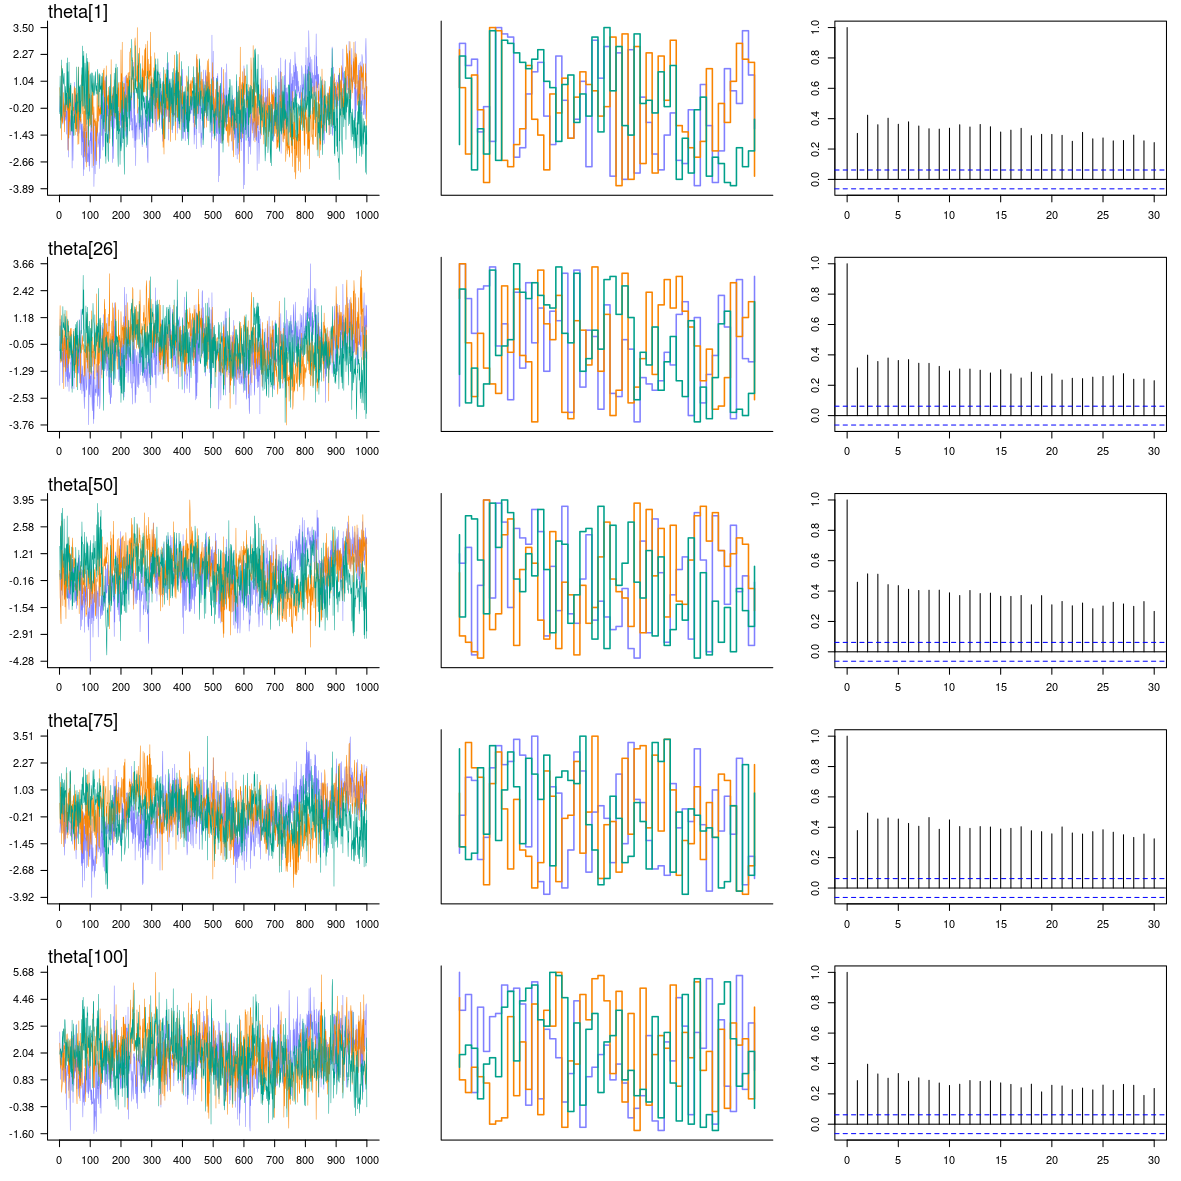
\includegraphics[width=1\linewidth]{SOLV_CE_J100_Ndata10_theta}
	%
	\caption[Second-Order latent variable model (SOLV). Sample size $100$, replica number $10$. Centered parametrization. Highest-order dimension. Trace, trank and auto-correlation plots.]%
	{Second-Order latent variable model (SOLV). Sample size $100$, replica number $10$. Centered parametrization. Highest-order dimension: (Left) trace plot, (Middle) trank plot, (Right) auto-correlation plot.}
	\label{fig:SOLV_CE_chains3}
\end{figure}
%
\begin{figure}[H]
	\centering
	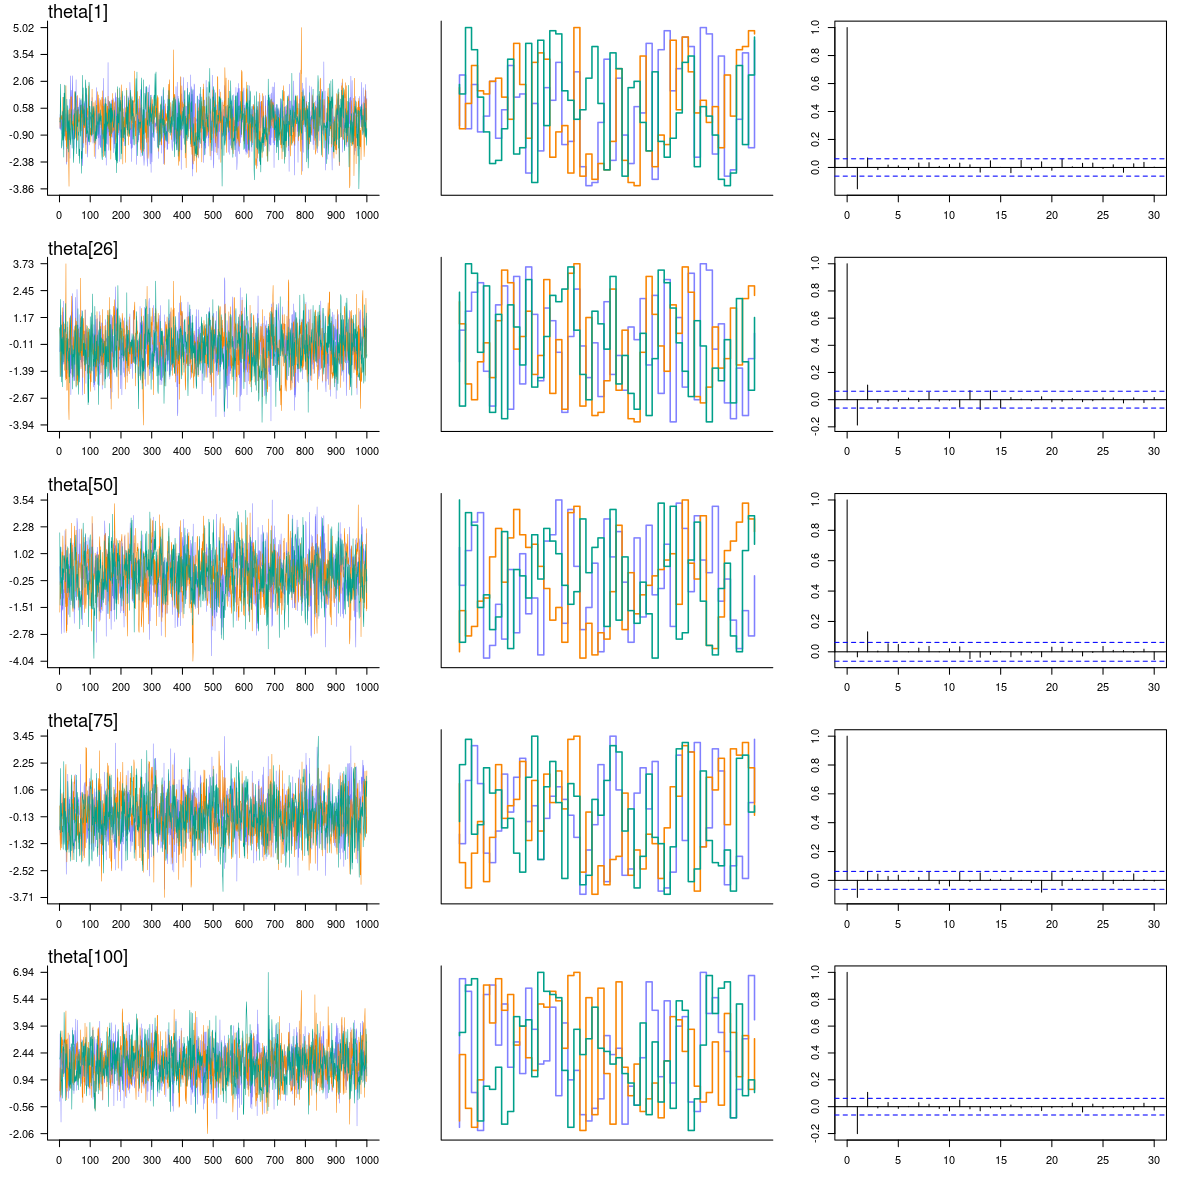
\includegraphics[width=1\linewidth]{SOLV_NC_J100_Ndata10_theta}
	%
	\caption[Second-Order latent variable model (SOLV). Sample size $100$, replica number $10$. Non-centered parametrization. Highest-order dimension. Trace, trank and auto-correlation plots.]%
	{Second-Order latent variable model (SOLV). Sample size $100$, replica number $10$. Non-centered parametrization. Highest-order dimension: (Left) trace plot, (Middle) trank plot, (Right) auto-correlation plot.}
	\label{fig:SOLV_NC_chains3}
\end{figure}
%
\begin{figure}[h]
	\centering
	\begin{subfigure}
		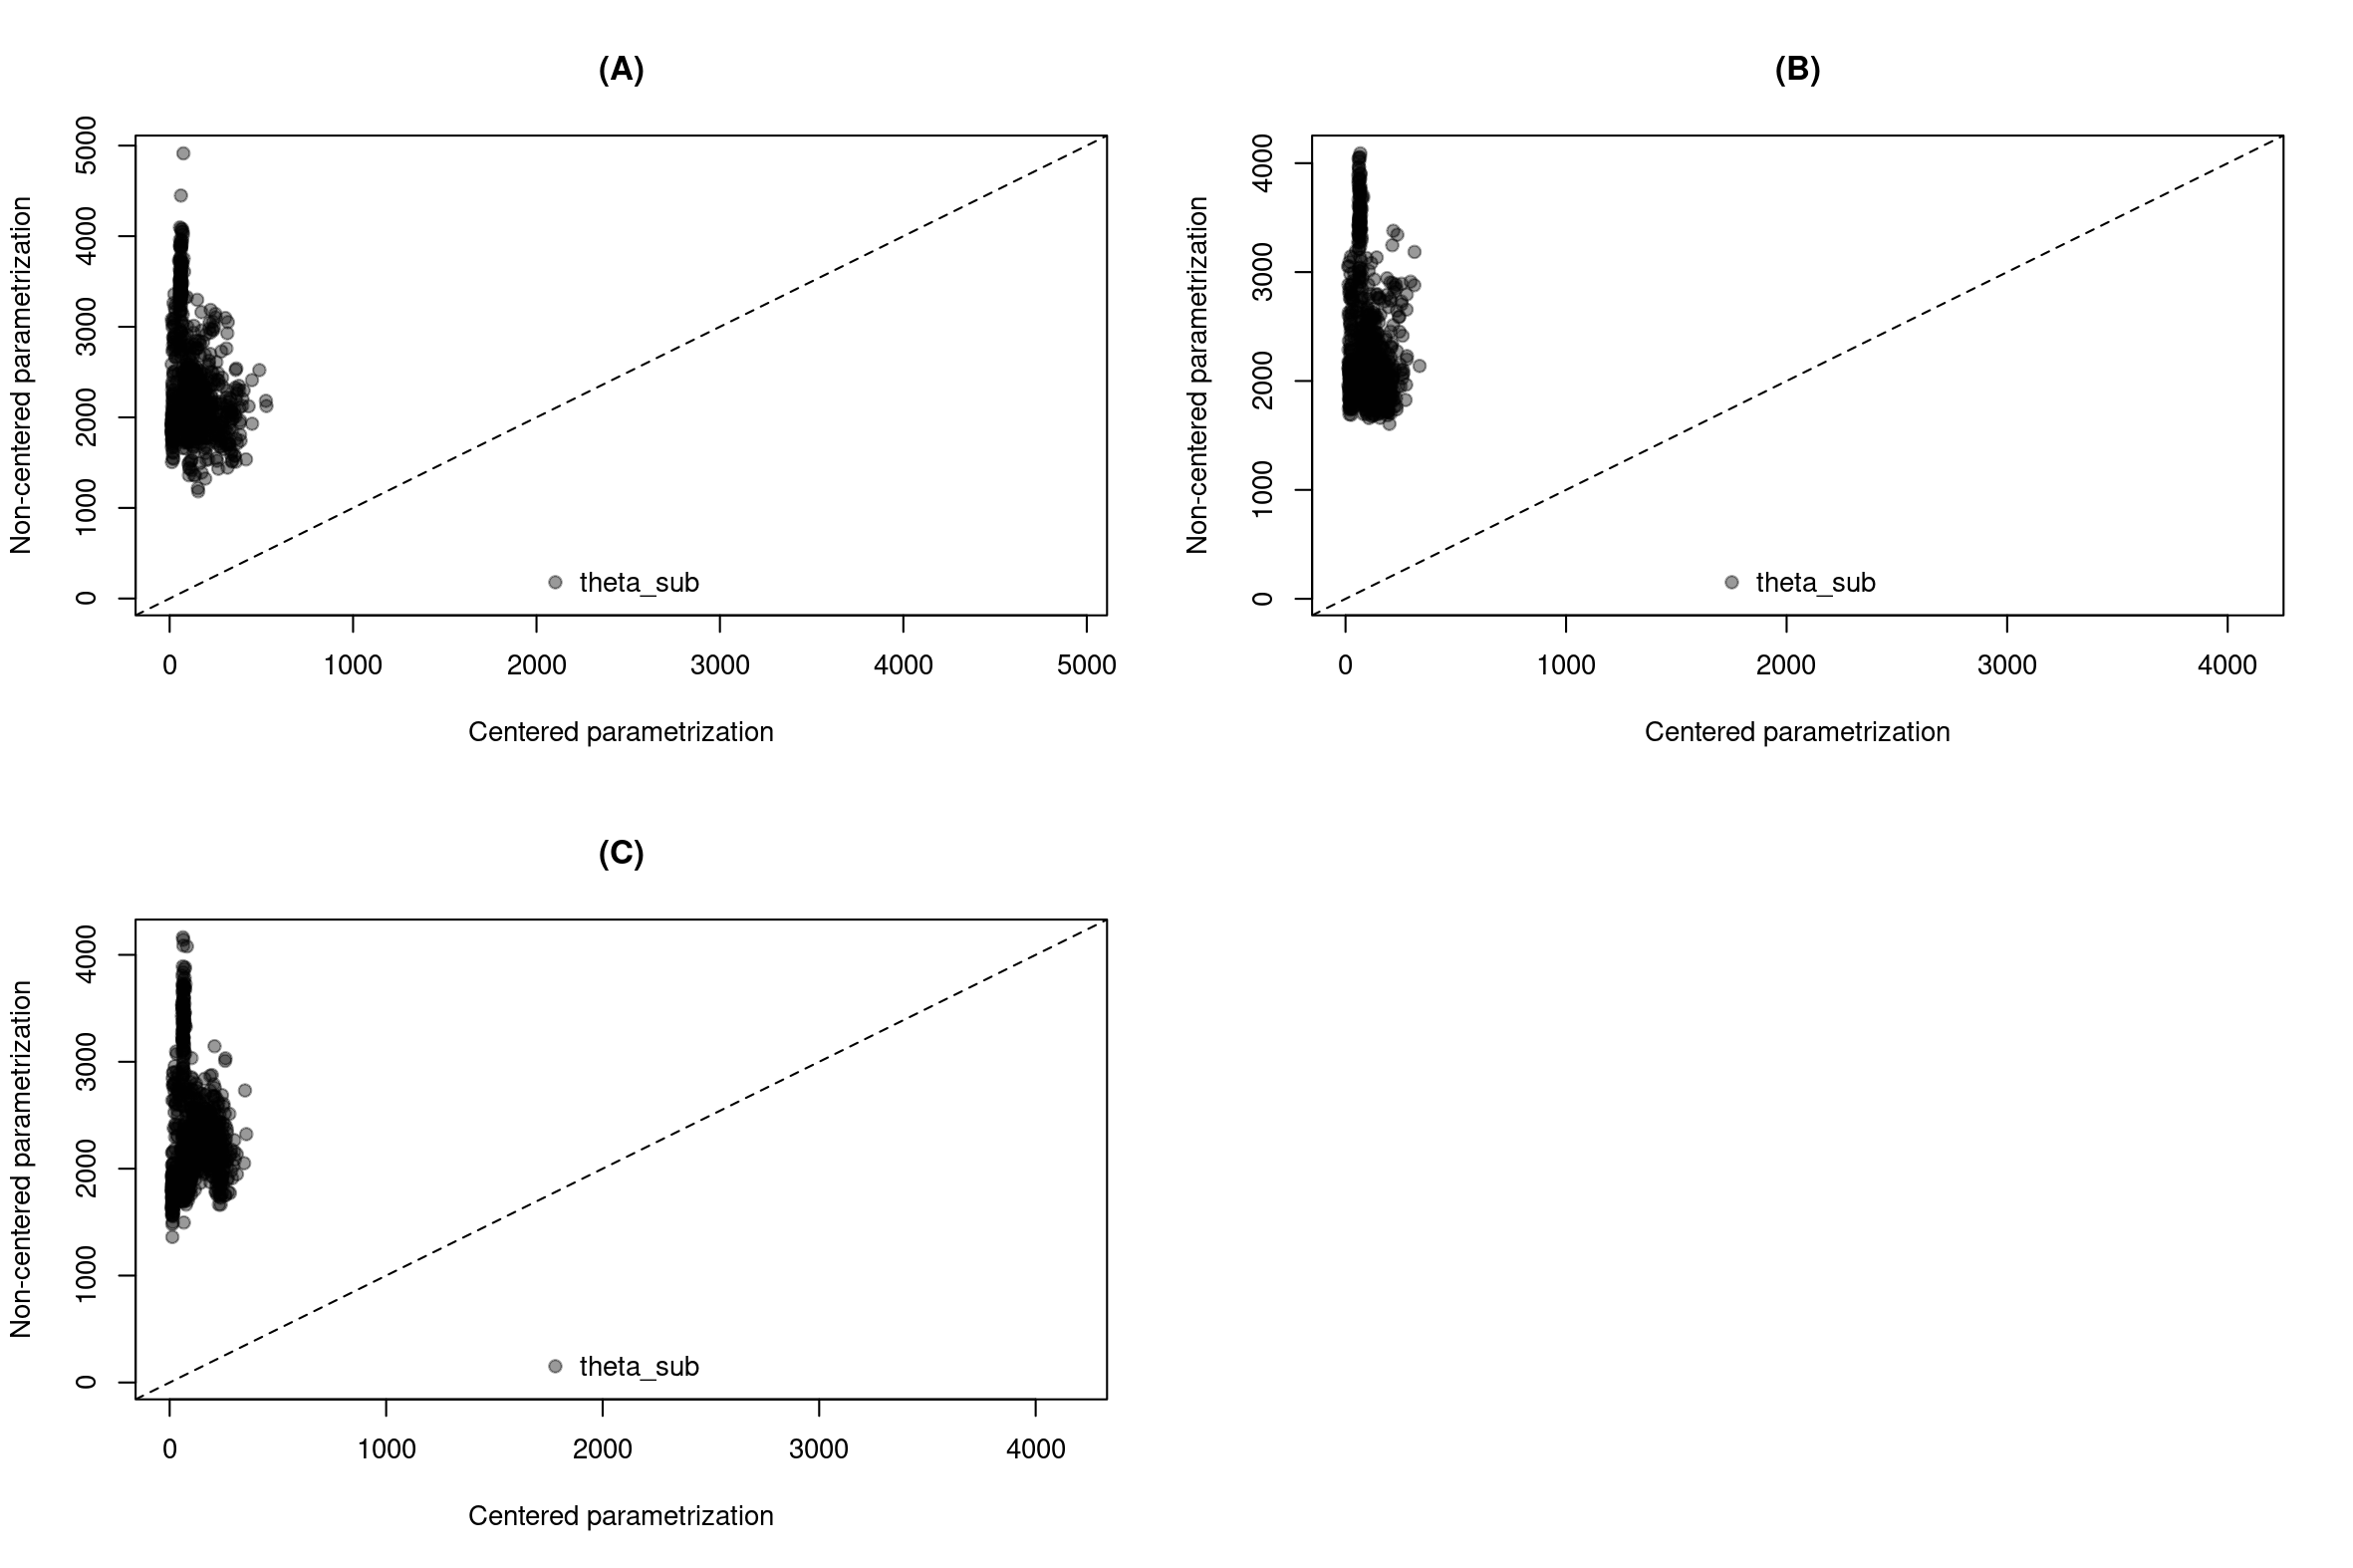
\includegraphics[width=1\linewidth]{FOLV_100_neff3}
	\end{subfigure}
	%
	\begin{subfigure}
		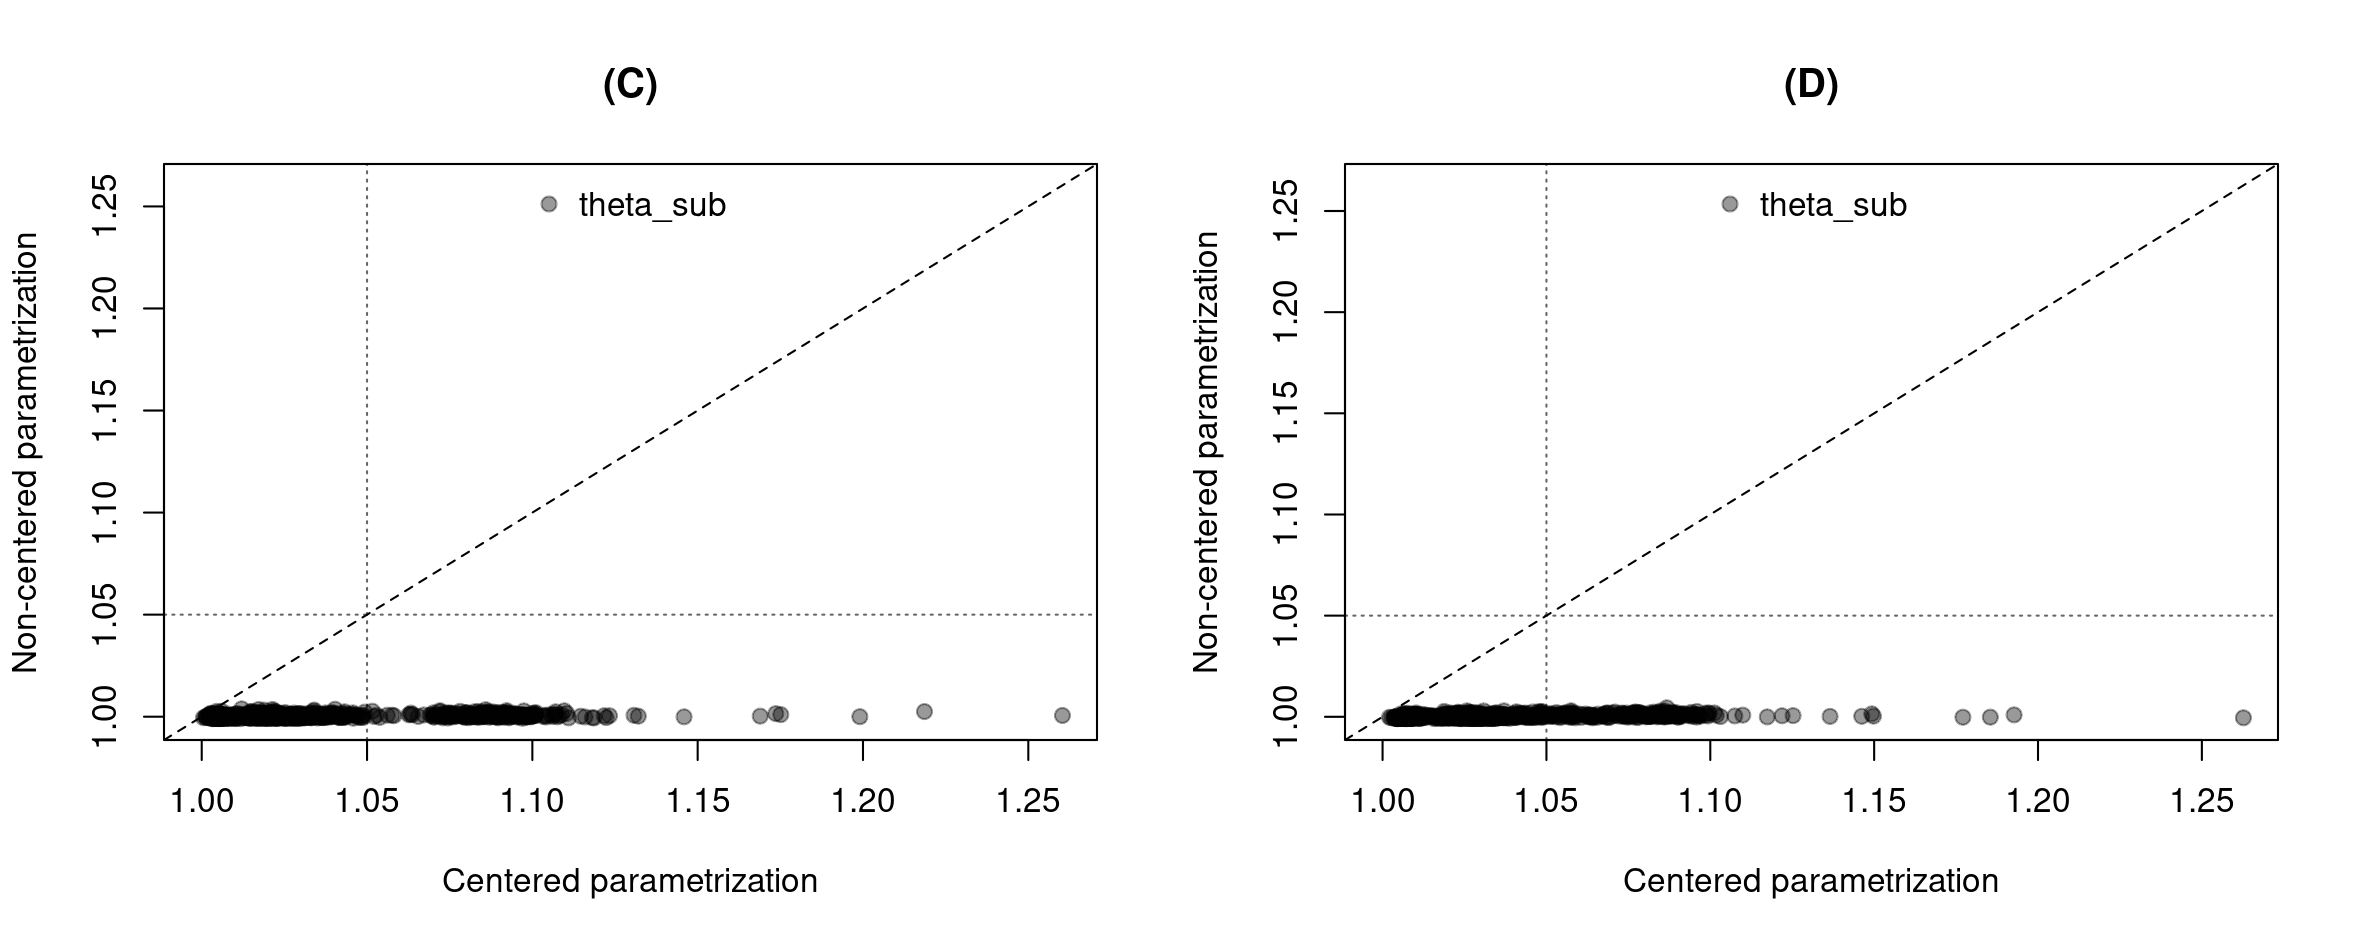
\includegraphics[width=1\linewidth]{FOLV_100_Rhat3}
	\end{subfigure}
	%
	\caption[First-order latent variable model (FOLV). Sample size $100$, all replicas. CP and NCP comparison plot.]%
	{First-order latent variable model (FOLV). Sample size $100$, all replicas. CP and NCP comparison plot. (A) \texttt{n\_eff} for the first sub-dimension. (B) \texttt{n\_eff} for the second sub-dimensions. (C) \texttt{Rhat} for the first sub-dimension. (D) \texttt{Rhat} for the second sub-dimensions. Diagonal discontinuous line describes equality between CP and NCP. Vertical and horizontal discontinuous lines is set at \texttt{Rhat}$=1.05$. }
	\label{fig:FOLV_stat3}
\end{figure}
%
\begin{figure}[h]
	\centering
	\begin{subfigure}
		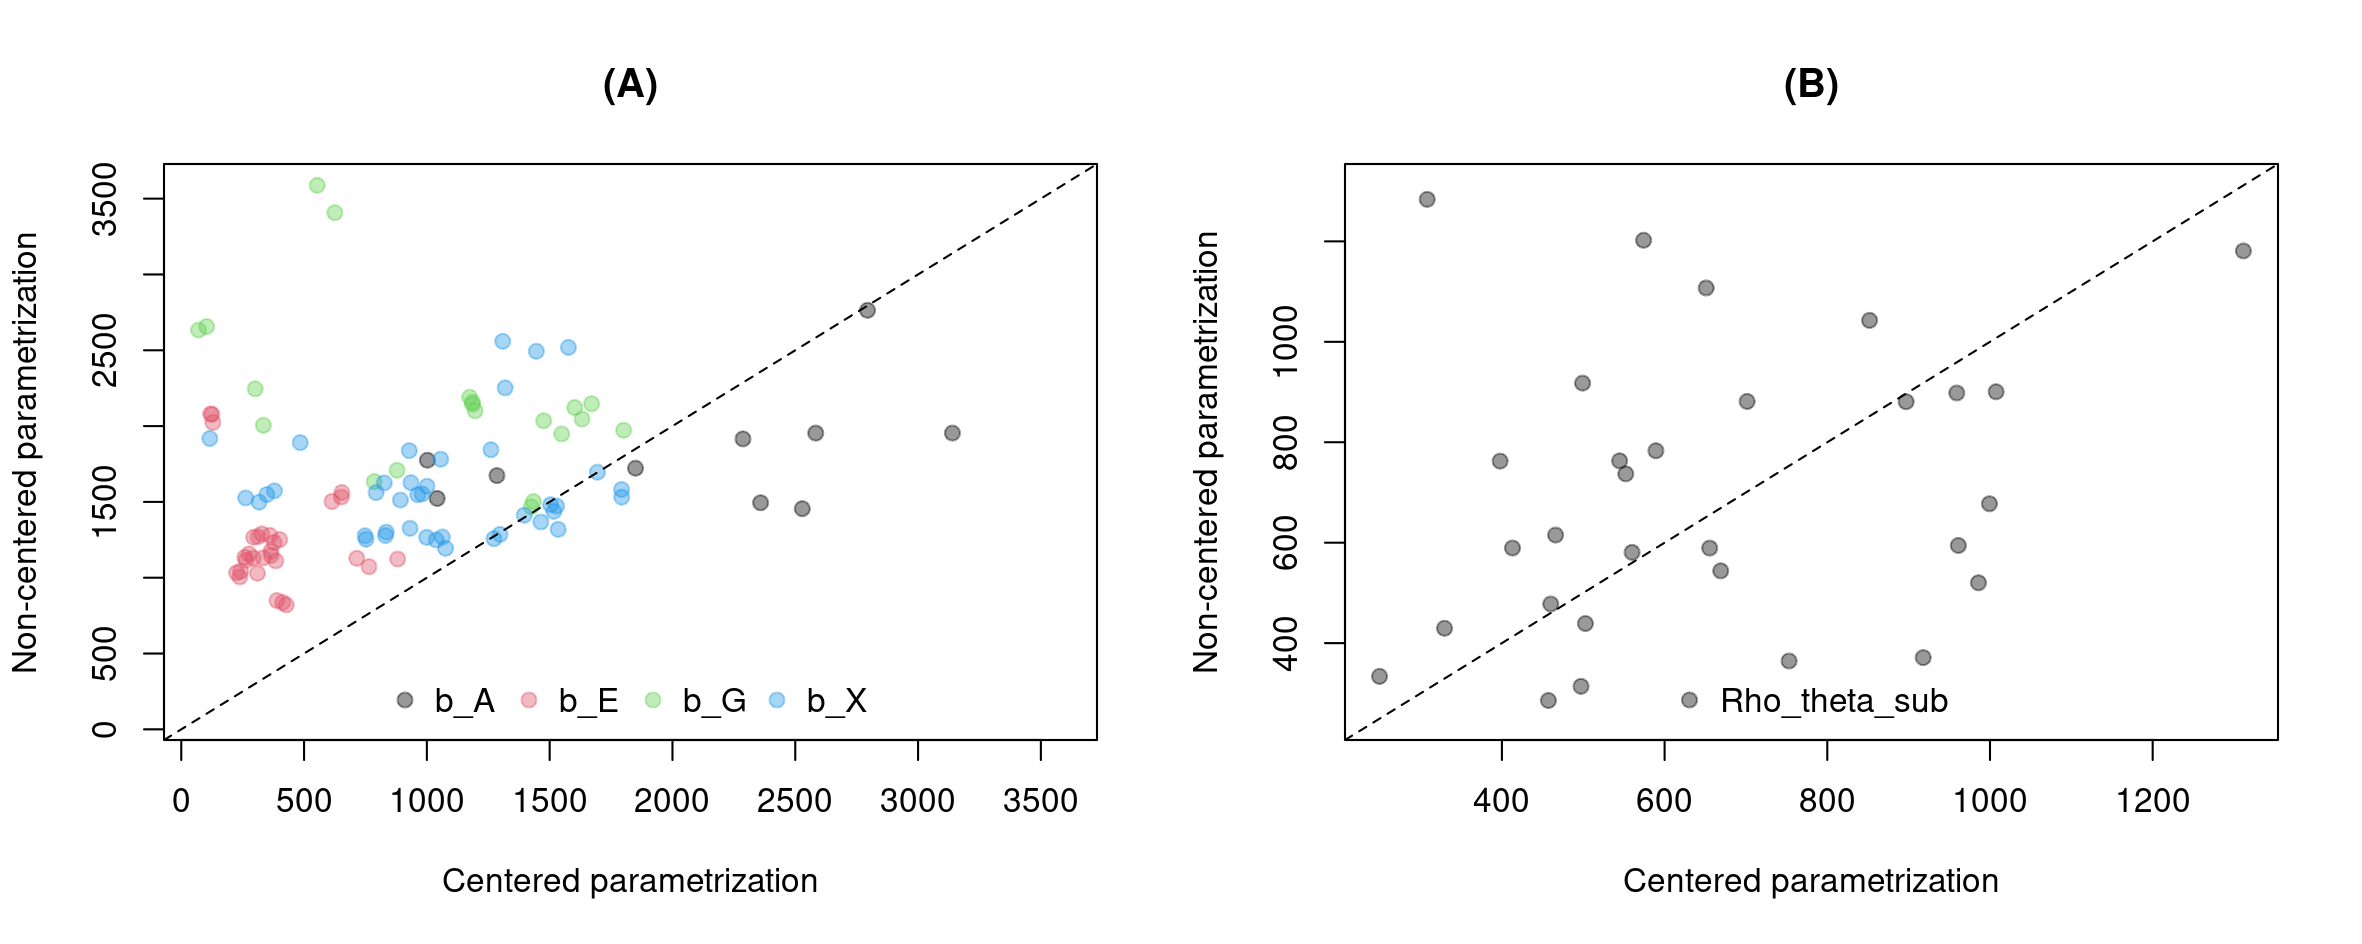
\includegraphics[width=1\linewidth]{FOLV_100_neff2}
	\end{subfigure}
	%
	\begin{subfigure}
		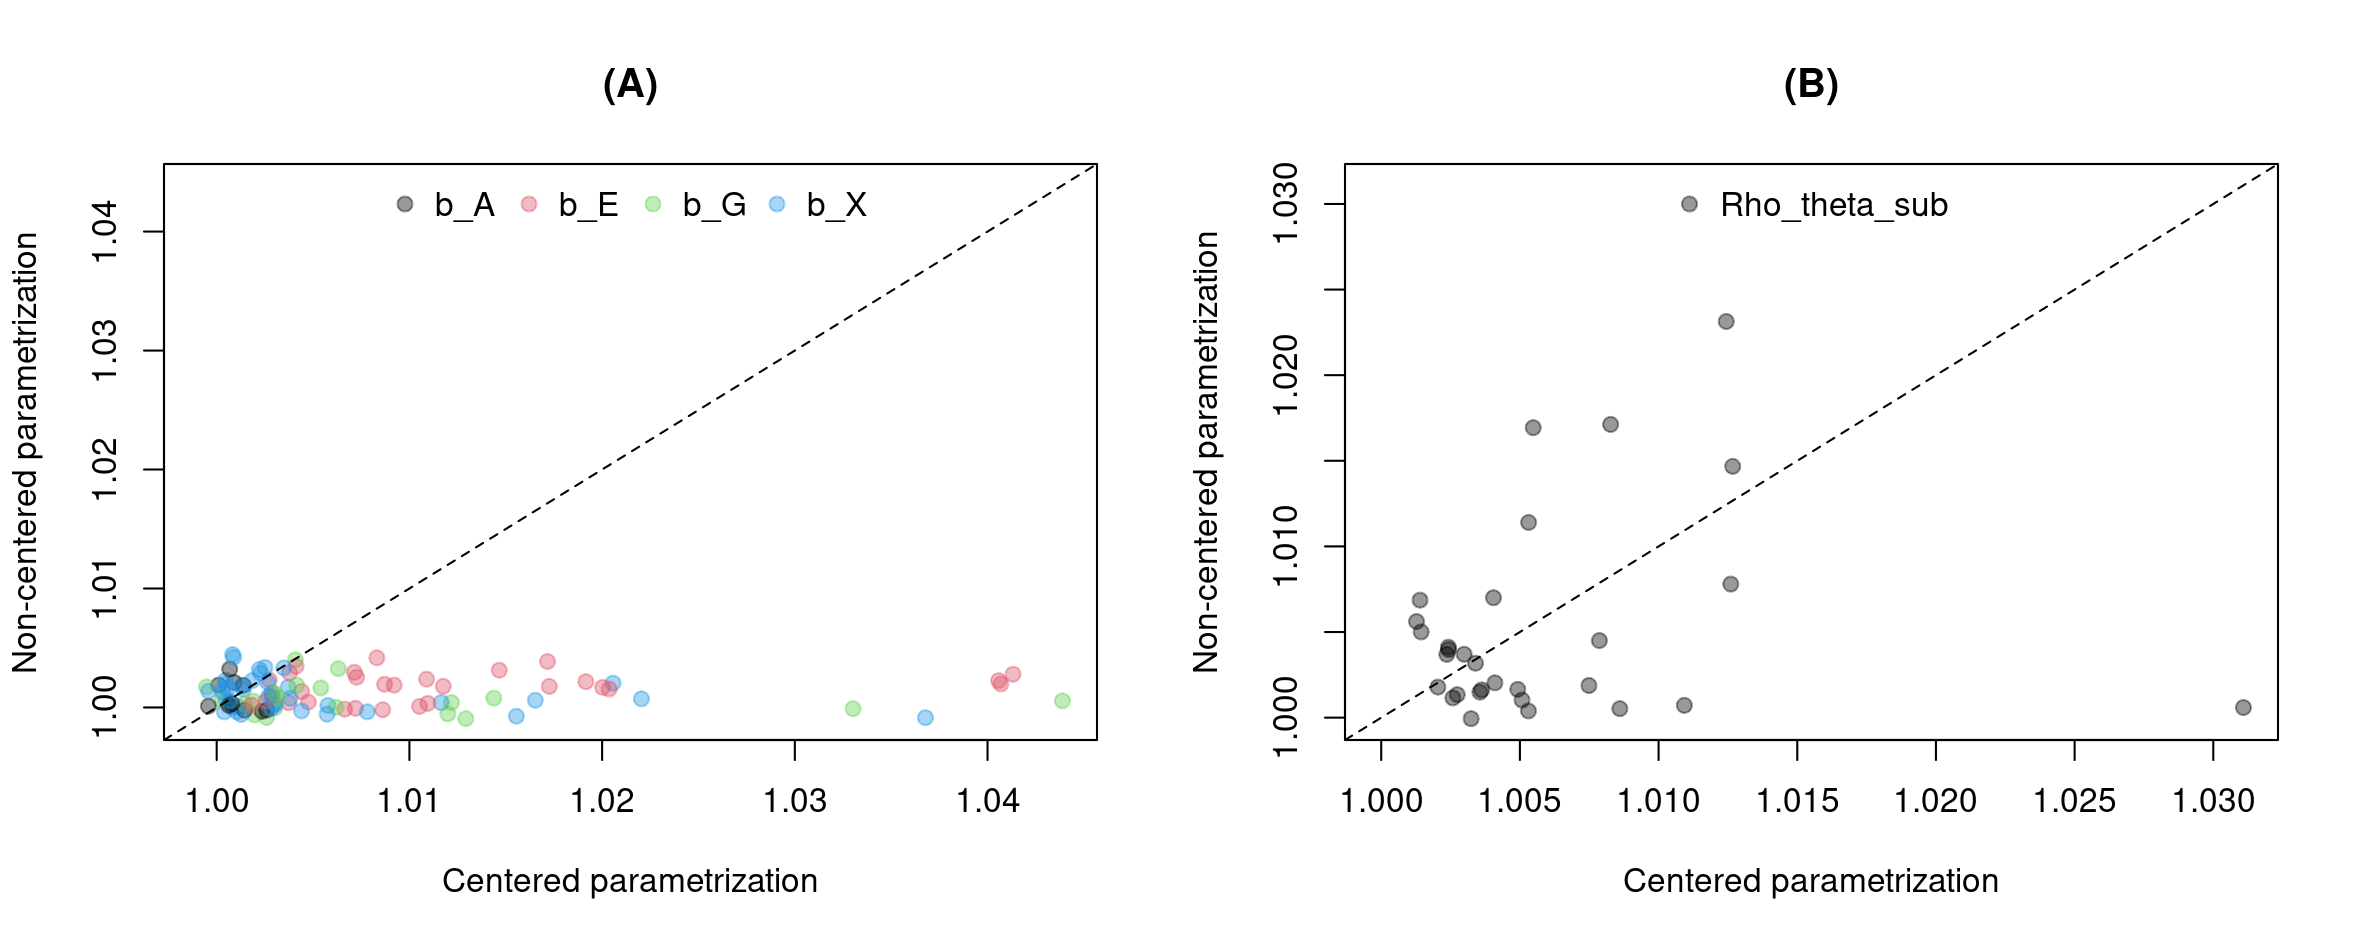
\includegraphics[width=1\linewidth]{FOLV_100_Rhat2}
	\end{subfigure}
	%
	\caption[First-order latent variable model (FOLV). Sample size $100$, all replicas. CP and NCP comparison plot.]%
	{First-order latent variable model (FOLV). Sample size $100$, all replicas. CP and NCP comparison plot. (A) \texttt{n\_eff} for regression parameters. (B) \texttt{n\_eff} for correlations among sub-dimensions. (C) \texttt{Rhat} for regression parameters. (D) \texttt{Rhat} for correlations among sub-dimensions. Diagonal discontinuous line describes equality between CP and NCP. Vertical and horizontal discontinuous lines is set at \texttt{Rhat}$=1.05$. }
	\label{fig:FOLV_stat2}
\end{figure}
%
\begin{figure}[h]
	\centering
	\begin{subfigure}
		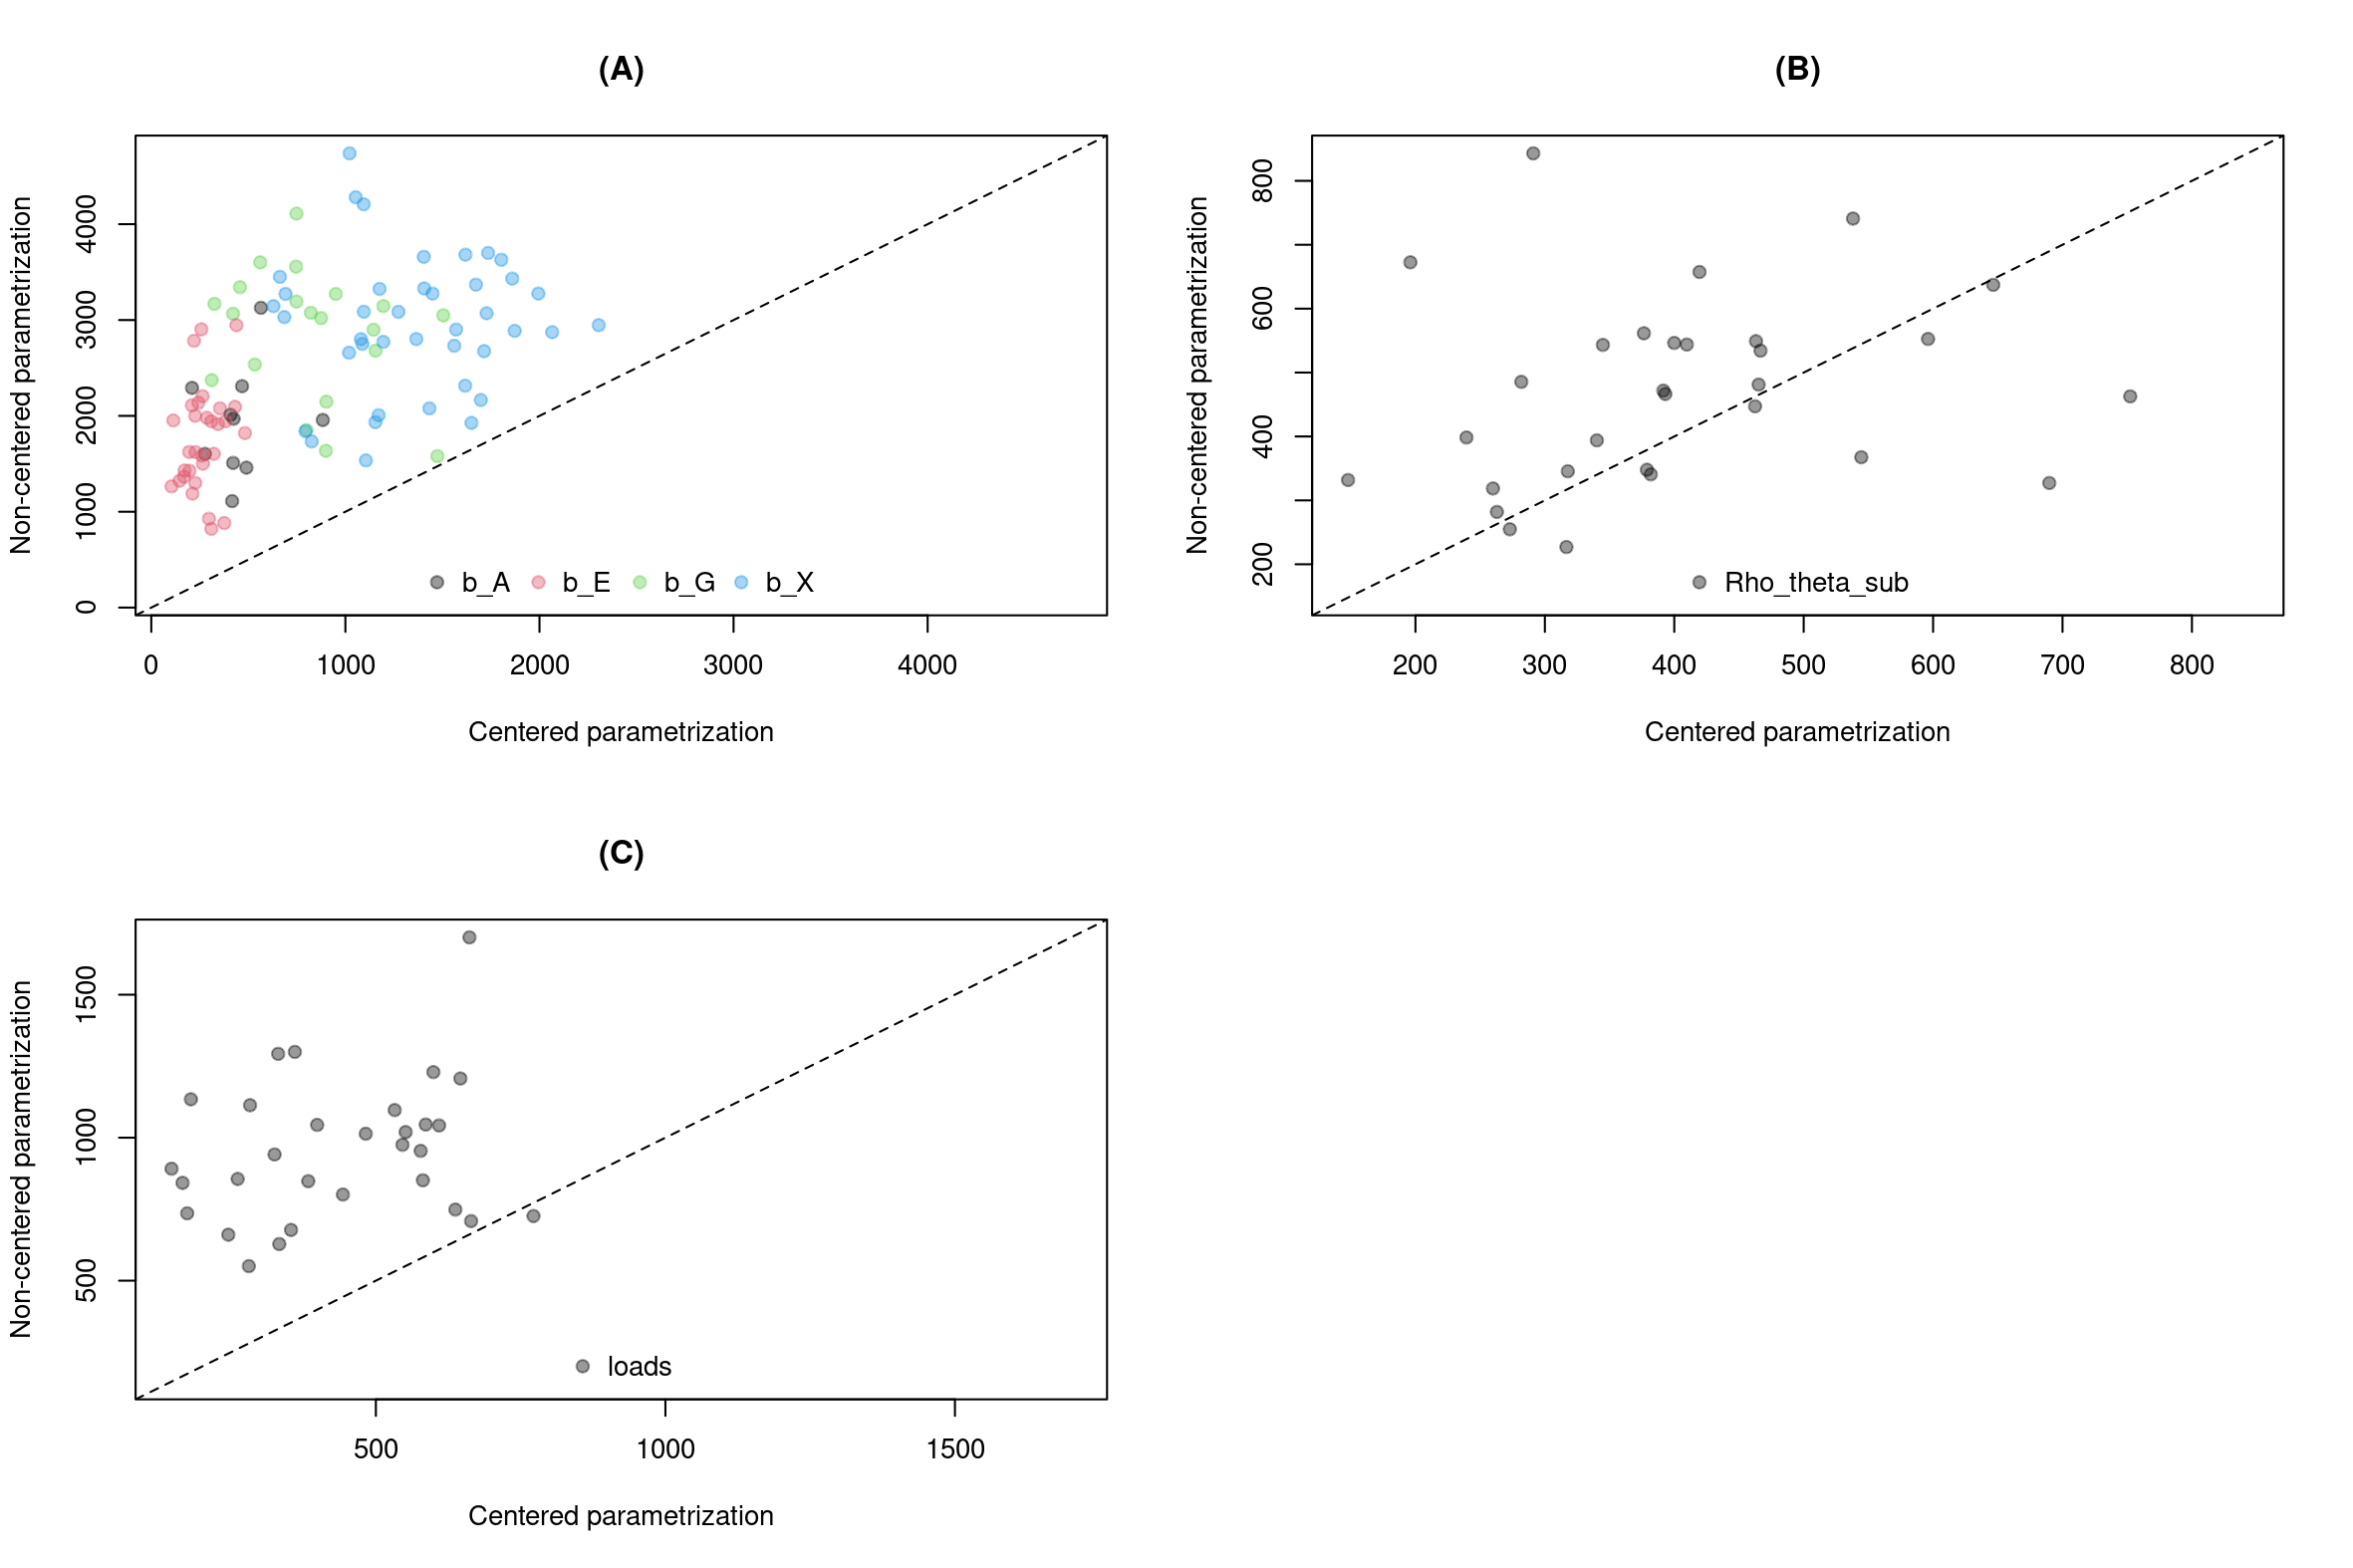
\includegraphics[width=0.48\linewidth]{SOLV_100_neff2}
	\end{subfigure}
	%
	\begin{subfigure}
		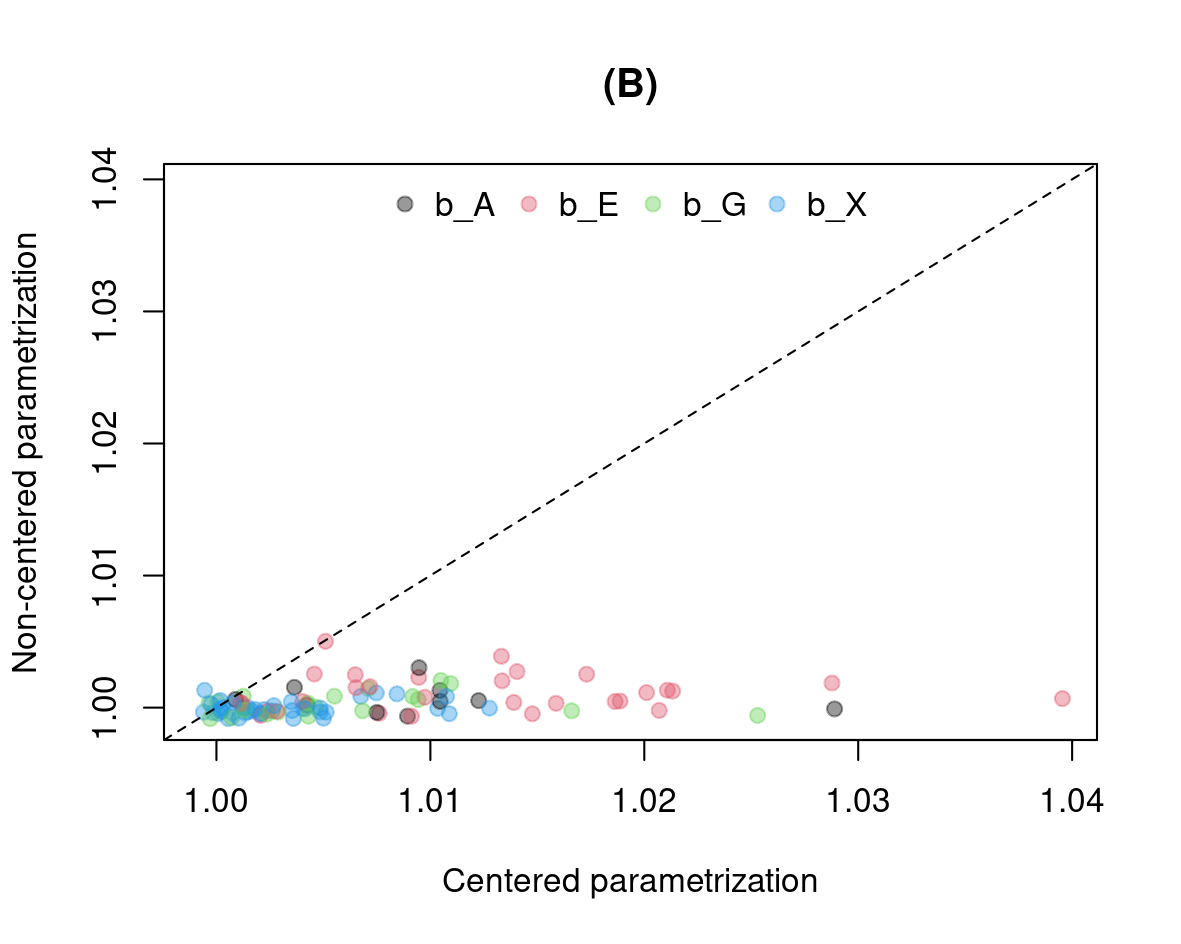
\includegraphics[width=0.48\linewidth]{SOLV_100_Rhat2}
	\end{subfigure}
	%
	\caption[Second-order latent variable model (SOLV). Sample size $100$, all replicas. CP and NCP comparison plot.]%
	{Second-order latent variable model (SOLV). Sample size $100$, all replicas. CP and NCP comparison plot. (A) \texttt{n\_eff} for regression parameters. (B) \texttt{Rhat} for the first sub-dimension. (D) \texttt{Rhat} for the second sub-dimensions. Diagonal discontinuous line describes equality between CP and NCP. Vertical and horizontal discontinuous lines is set at \texttt{Rhat}$=1.05$. }
	\label{fig:SOLV_stat1}
\end{figure}
%
\begin{figure}[h]
	\centering
	\begin{subfigure}
		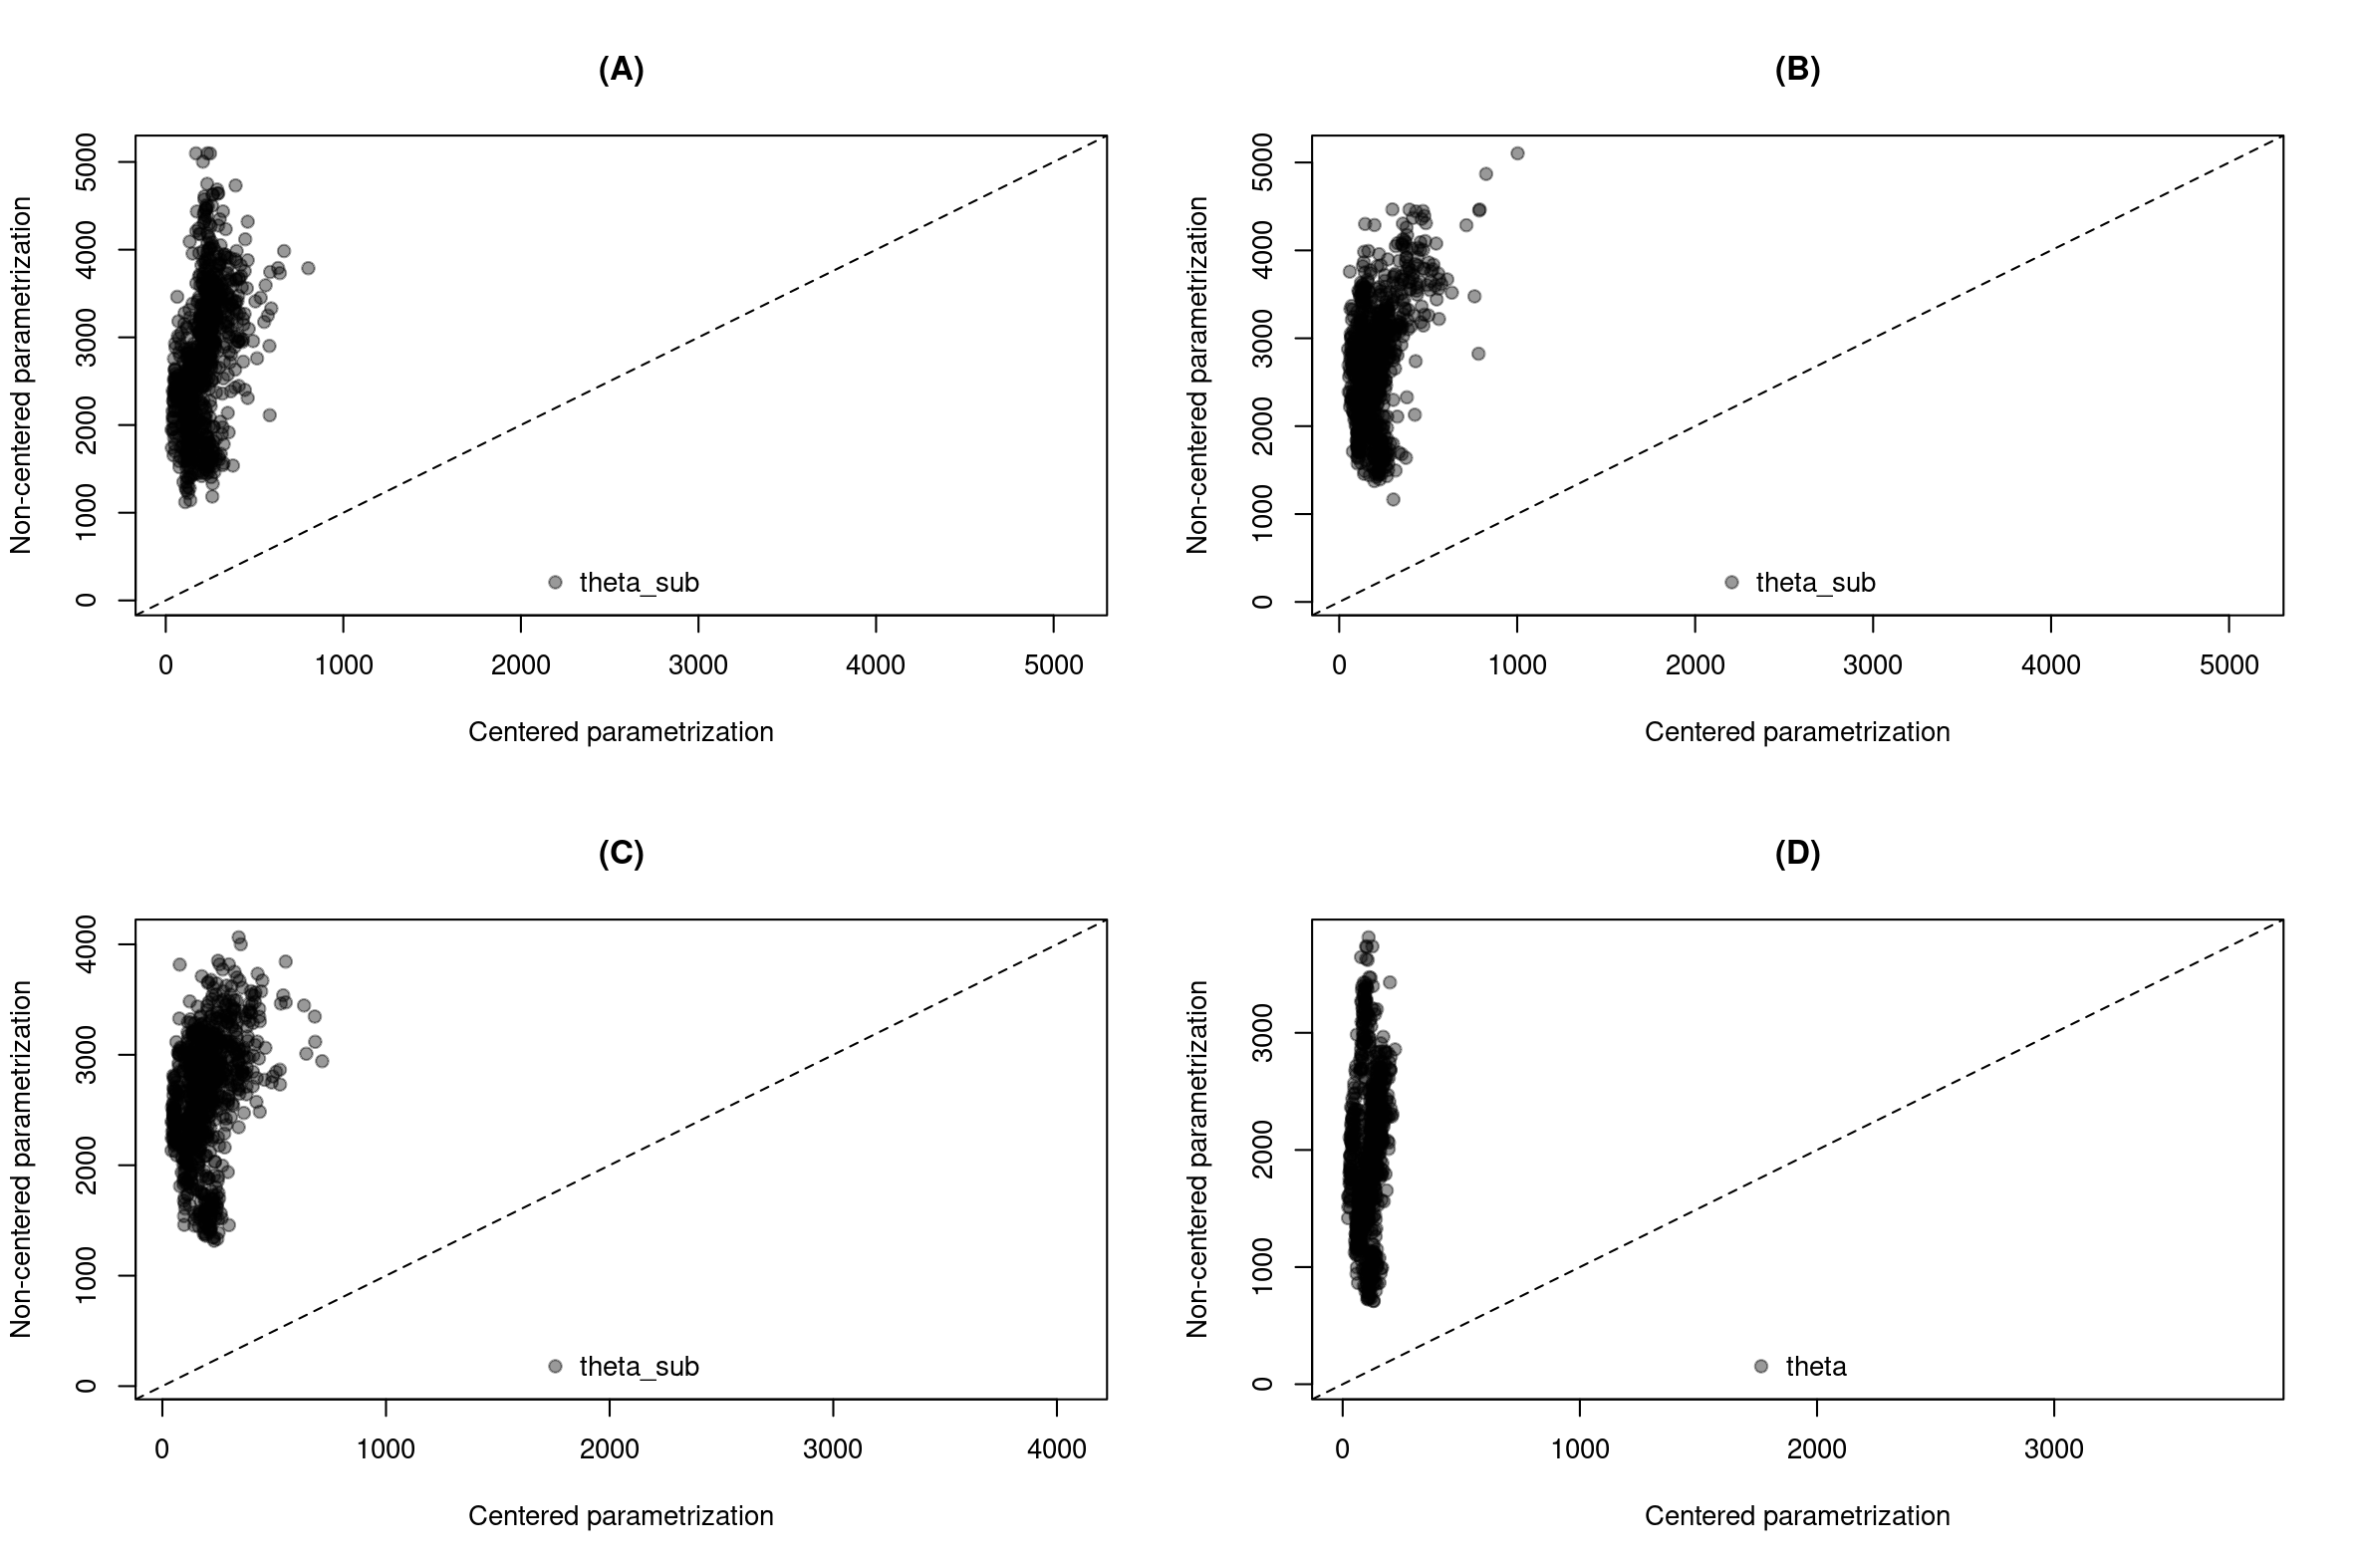
\includegraphics[width=1\linewidth]{SOLV_100_neff3}
	\end{subfigure}
	%
	\begin{subfigure}
		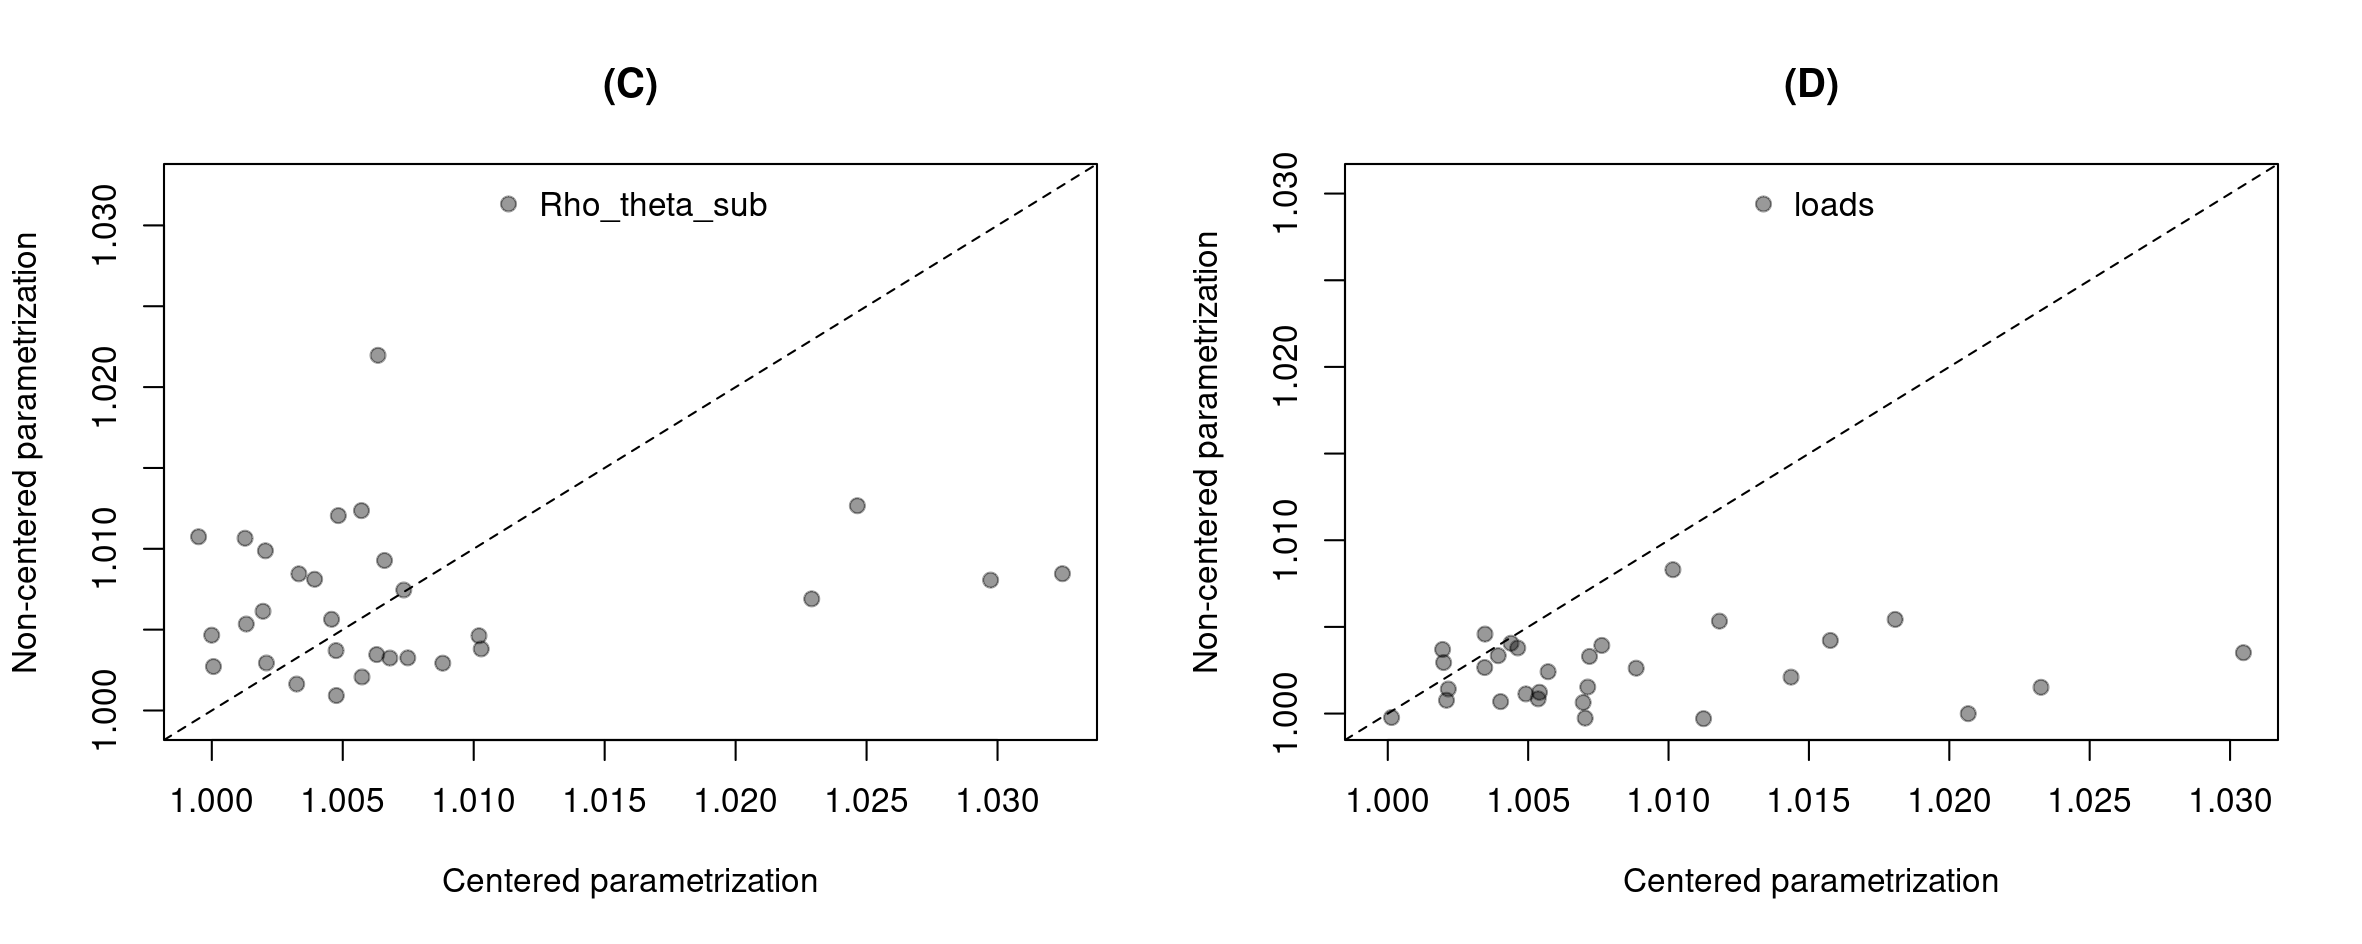
\includegraphics[width=1\linewidth]{SOLV_100_Rhat3}
	\end{subfigure}
	%
	\caption[Second-order latent variable model (SOLV). Sample size $100$, all replicas. CP and NCP comparison plot.]%
	{Second-order latent variable model (SOLV). Sample size $100$, all replicas. CP and NCP comparison plot. (A) \texttt{n\_eff} for the correlations among sub-dimension. (B) \texttt{n\_eff} for the loadings. (C) \texttt{Rhat} for the correlation among sub-dimensions. (D) \texttt{Rhat} for the loadings. Diagonal discontinuous line describes equality between CP and NCP. Vertical and horizontal discontinuous lines is set at \texttt{Rhat}$=1.05$. }
	\label{fig:SOLV_stat2}
\end{figure}